\documentclass[11pt]{article}

\usepackage[margin=1in]{geometry}
\usepackage[T1]{fontenc}
\usepackage{amsmath}
\usepackage{amssymb}
\usepackage{amsthm}
\usepackage{graphicx}
\usepackage{float}
\usepackage{booktabs}
\usepackage{tabularx}
\usepackage{algorithm}
\usepackage{algpseudocode}
\usepackage{tikz}
\usetikzlibrary{arrows.meta,positioning,calc,fit,shapes.geometric}
\usepackage[font={small,sf},labelfont={bf,sf},labelsep=period,margin=8pt]{caption}
\usepackage[hidelinks]{hyperref}
\usepackage{url}
\usepackage{siunitx}
\usepackage{microtype}
\usepackage[numbers,sort&compress]{natbib}

\newtheorem{theorem}{Theorem}
\newtheorem{corollary}[theorem]{Corollary}
\newtheorem*{fact}{Fact}
\newtheorem*{remark}{Remark}

\newcommand{\kasparhft}{\textsc{Kaspar-HFT}}
\newcommand{\shadowpov}{\textsc{Shadow-POV}}

\title{Two Threads Beat One, and the Thread Hop Is a Wash\\
Under Hawkes Arrivals:\\
A Closed-Form and Empirical Case for Multi-Actor HFT Pipelines}
\author{Vincent Mayeski\thanks{M2 Tech (16425640 Canada Inc.), Montreal. \texttt{v@m2te.ch}}}
\date{Draft v2, September 2026}

\begin{document}
\maketitle

\begin{abstract}
The received wisdom in high-frequency-trading (HFT) system design is that the entire hot path --- SBE decode, order-book application, strategy touch, order construction --- should live on a single-thread event loop, because every additional thread hop adds real wall-clock latency. This paper shows that received wisdom is wrong on real CME Market Data Platform version 3 (MDP3) packet flow, and reports two contrarian conclusions.

\textbf{First: the thread-hop cost is a wash.} The received single-thread wisdom assumes that a $\sim 1.7\,\mu\mathrm{s}$ one-way async mailbox hop (\citet{mayeski_fastsend} Table 4; the fast\_send paper's $3.4\,\mu\mathrm{s}$ round-trip halved) is a material addition to end-to-end latency. On real Hawkes-clustered CME MDP3 packet arrivals, the observed cluster-wait tail is one to two orders of magnitude larger than that per-hop cost in both service-floor regimes tested so far, so the hop is not a first-order effect. The single-thread objection --- ``every hop is a fixed tax that no benefit can overcome'' --- is empirically wrong on this class of feed.

\textbf{Second: two threads beat one on the tail at the cost of one hop on the median.} Splitting a service task into two half-length actors on separate threads joined by one $1.7\,\mu\mathrm{s}$ mailbox hop cuts the corpus-median $p_{99}$ tail excess by more than half while adding exactly $h$ to the median, a favourable trade for any operator who weights a microsecond of tail at $\gtrsim 0.15$ of a microsecond of median, at every service floor $T \gtrsim 2 h$. The exact numerical corpus medians come from the $T \in \{2, 4, 8, 16, 32\}\,\mu\mathrm{s}$ sweep now in flight; the tables in Section~\ref{sec:results} will carry the final numbers. The same pattern generalises to an $N$-stage series tandem: the end-to-end wait is at most $1/N$ of the single-stage wait plus $(N-1)h$, at every quantile and on every sample path, capped by the number of natural cut points in the decode chain (four or five on CME MDP3).

The effect is entirely arrival-law-driven: under a rate-matched Poisson null on the same arrival count, both wins vanish and the multi-actor architecture strictly loses. Two closed-form results anchor the mechanism (a burst-limit throughput identity, and an exact pathwise reduction of the deterministic-service tandem to a single server that yields the $1/N$ bound); a fork-based literature search over foundational tandem theory, Hawkes-adjacent queueing, and empirical HFT/RPC work found no direct prior art on either the theoretical statement or the empirical calibration. Companion code contains the message-tape parser, the per-window packet-Hawkes fitter, and the tandem Lindley simulator.
\end{abstract}

\clearpage
\tableofcontents
\clearpage

% =====================================================================

\section{Introduction}
\label{sec:intro}

\subsection{The design choice, and the safe default}
\label{sec:intro-debate}

The design of the ingress-to-order pipeline in a high-frequency trading system is a choice between two archetypes: the single-threaded event loop that processes every step of every message on one core (SBE decode, book application, strategy evaluation, order construction, all under one call chain, taking a total service time we denote $T$), and the multi-actor pipeline in which those steps are split across $N$ separate actors, each on its own thread with its own mailbox, connected by $N-1$ explicit hops whose per-hop wall-clock cost we denote $h$. It is not really a debate: almost everyone in the low-latency HFT community is in the single-thread camp, and single-threaded is generally viewed as the safe choice. The argument for it cites the cost of a mailbox hop --- typically a mailbox enqueue plus a cache-line transfer between the sender's core and the receiver's core, plus the cost of the receiver being scheduled or spinning --- and holds that $(N-1) h$ adds directly to every message's end-to-end latency, so every extra stage in the pipeline is a fixed tax that no throughput or tail benefit can overcome.

That argument implicitly assumes an arrival process for which single-server throughput $1/T$ is comfortably larger than the peak arrival rate. On CME MDP3 the arrival process is strongly self-exciting: packets arrive in Hawkes-clustered bursts \citep{filimonovsornette2012,hardimanbercotbouchaud2013,bacry2015review}. During such bursts the instantaneous arrival rate transiently exceeds the single-thread event loop's service rate $1/T$, and cluster-induced queueing accumulates a tail that dwarfs $h$ by one to two orders of magnitude. This paper's central empirical observation, on a 23-session interim subset of a 281-session NQ front-month corpus whose full sweep is in flight, is that this cluster tail is what dominates observed end-to-end latency: the $99$th-percentile latency ($p_{99}$) of a $T = 10\,\mu\mathrm{s}$ constant-service queue driven by real packet arrivals is four times the service floor at the corpus-median window and larger still in the high-clustering half of the windows. Under a rate-matched Poisson null of the same arrival count the $p_{99}$ equals the median; the tail is entirely a Hawkes-cluster effect.

Given that the tail is cluster-driven, the natural question is whether splitting the pipeline into $N > 1$ stages --- each running as an independent actor on its own core, with per-stage service $T/N$, so that the tail-driving cluster-wait is now split across $N$ smaller queues --- reduces the tail. If it does, and if the additional median cost $(N - 1) h$ is small relative to the tail savings, the multi-actor architecture is the better trade for any tail-weighted operator, and the single-thread default is displaced for HFT workloads specifically. All symbols in this paragraph are gathered in the notation table of Section~\ref{sec:notation}.

\subsection{Prior recommendations for single-thread hot paths}
\label{sec:intro-singlethread-priors}

The single-thread rule has a specific lineage in the low-latency-systems community, and we name that lineage here because the paper is arguing against it directly. In reverse chronological order, the lineage has three layers: the HFT-specific codification of the last decade, the general low-latency-systems and event-driven-server culture from which HFT inherited it, and one prominent published counter-argument that the field discarded.

\paragraph{Modern HFT-community codification (2010--present).} The founding statement of the current HFT-community formulation is Thompson's Single Writer Principle \citep{thompson2011singlewriter} --- ``a single-writer design consistently outperforms a `properly' lock-free or wait-free multi-writer design on most realistic workloads'' --- motivated by and applied in the LMAX Exchange architecture \citep{fowler2011lmax,lmaxdisruptor}. Rigtorp's widely cited low-latency tuning guide \citep{rigtorp_lowlatency} formalises the operational rule (``run a single thread in \texttt{SCHED\_OTHER} per core and use busy waiting/polling''), and Chronicle Software's public engineering materials \citep{chronicle_fasttrading} adopt the same architecture for market-data connectors (``within a single event loop \ldots busy-spinning and affinity locks''), pinning Chronicle Queue's design to a single writer per queue. The Aeron messaging library \citep{aeron} inherits the same lineage. The academic side is thinner, but \citet{kwan2023hftpatterns} codify the pattern as the standard low-latency-HFT design pattern, and recent practitioner posts \citep{hu2024sequencer} restate it explicitly (``all critical trading logic runs in a single-threaded event loop, eliminating context switches and lock contention entirely''). Inside HFT specifically, the same recommendation has been reinforced by two decades of private prop-trading arms-race practice among the Chicago desks (Getco, Jump, Optiver, DRW; late 2000s), reported second-hand in industry retrospectives but without an open-literature reference.

\paragraph{Older event-driven-server lineage (1995--2010).} HFT did not invent this rule; it inherited it from the event-driven-server culture. The single-threaded event loop as an architectural pattern dates at least to Schmidt's Reactor pattern \citep{schmidt1995reactor} in the mid-1990s. It was sharpened by Kegel's C10K essay \citep{kegel1999c10k}, which named the OS thread-per-connection model as the bottleneck of scalable network servers and argued for event-driven designs. The pattern went mainstream in production with Sysoev's nginx web server \citep{sysoev2004nginx}, whose single-threaded worker process is explicitly justified as context-switch avoidance, and later with Dahl's Node.js runtime \citep{dahl2009nodejs}, which pushed the single-threaded event loop into ordinary application code.

\paragraph{Pro-pipelining minority --- outside HFT.} A legitimate multi-decade pro-pipelining tradition exists in the datacenter and networking-systems literature; it has been the field's non-single-thread minority throughout the period covered by the previous two paragraphs. The earliest prominent published argument is the Staged Event-Driven Architecture (SEDA) of \citet{welsh2001seda}, which advocated exactly the multi-stage pipeline of independently scheduled event handlers that the present paper's tandem design revives. Welsh's 2010 retrospective \citep{welsh2010retrospective} is often cited as a walk-back to single-thread, but it is actually a hedged pro-pipelining recommendation: it advocates decoupling stages from thread pools, grouping multiple stages within a single thread-pool domain where latency is critical, and putting a separate thread pool and queue in front of any stage with long or nondeterministic runtime --- effectively the present paper's design rule in different vocabulary. Beyond SEDA the pro-pipelining tradition includes the Click Modular Router \citep{kohler2000click} for staged packet processing; Naiad \citep{murray2013naiad} for low-latency dataflow; Snap \citep{marty2019snap} for Google's multi-engine network stack; and the datacenter microsecond-tail-latency scheduler line --- Shinjuku \citep{kaffes2019shinjuku}, Shenango \citep{ousterhout2019shenango}, Caladan \citep{fried2020caladan}, Perséphone \citep{delimitrou2021persephone} --- which argues for centralised multi-core dispatch specifically to control the microsecond-scale tail. Perséphone in particular is targeted at ``wide service-time distributions,'' the closest existing framing to our arrival-law claim; but the datacenter line frames the problem as heavy-tailed \emph{service}, not clustered \emph{arrivals}. DPDK explicitly supports both run-to-completion and pipeline modes and its documentation recommends pipeline mode ``if some set of packets require longer to process'' \citep{dpdk}. Inside HFT specifically the pro-pipelining position is rare in the open literature; an obscure Chinese patent \citep{cn105654383a} describing a pipelined FAST market-data decoder is a lonely commercial artefact of it.

None of the pro-pipelining sources above ties the design recommendation to Hawkes / self-exciting / near-critical arrival dynamics. The closest theoretical hooks are the MMPP-input tandem work of \citet{kimchydzinski2002mmpp} already cited in Section~\ref{sec:intro-priors} and the batch-arrival tandem phase-transition analysis of \citet{tandembatch2014}. The present paper's arrival-law-specific mechanism --- that the recommendation flips when arrivals are near-critically self-exciting --- remains uncontested by prior work.

Yours truly gets a footnote on that list, but with an important caveat.\footnote{A related author's-aside: the tail compression reported by this paper had in fact been observed empirically in production well before its mechanism was understood. Splitting a long task into shorter asynchronously connected stages was known to help the tail on a per-strategy basis in the author's own operational experience, and the working assumption at the time was that the single-thread camp must simply be writing faster inner-loop code --- not that the architectural recommendation was itself arrival-law-dependent. The present paper is the retrospective explanation of that anecdote.} An earlier paper by the present author \citep{mayeski_fastsend} did not argue for the single-thread principle in its own right. That paper is defensive rather than prescriptive: the actor model had long been dismissed as unsuitable for HFT because of asynchronous-dispatch overhead, and \texttt{fast\_send} is presented there as the mechanism that eliminates the overhead for co-located actors and thereby makes the actor model usable \emph{inside} a servicing chain that the received wisdom of the time had already placed on a single thread. The reference architecture in that paper --- reader $\to$ buffer via asynchronous \texttt{send}, decode/book/signal chain via \texttt{fast\_send} on one thread, signal $\to$ order-out via asynchronous \texttt{send} --- takes the collapsed single-thread servicing chain as the widely accepted design context of the time and delivers a way to compose it out of actors at zero context-switch cost. It does not compare single-thread against more-asynchronous topologies and pick single-thread; it takes the topology as given. The present paper is a retraction of that design context, not of the \texttt{fast\_send} mechanism: on Hawkes-clustered feeds, the aggregate servicing chain should be split into asynchronous stages once its total service time becomes long compared to the Hawkes-cluster tail. \texttt{fast\_send} remains the right mechanism for chaining actors that have been placed together on one thread; what changes is where the thread boundaries inside the servicing chain should sit. The corrected design rule is stated in Section~\ref{sec:conclusion}.

\subsection{What this paper does}
\label{sec:intro-plan}

We answer that question along three axes.

\begin{itemize}
    \item \textbf{Theory.} Two closed-form theorems (Section~\ref{sec:theory}) predict the pipeline behaviour. Theorem~\ref{thm:burst} shows that under any arrival process an $N$-stage tandem enjoys an $N$-factor throughput speedup on isolated bursts. Theorem~\ref{thm:reduction} shows that a deterministic-service tandem reduces exactly to a single server with the largest stage's service, and that the end-to-end wait is bounded pathwise by $1/N$ of the single-stage wait plus $(N-1)h$, at every quantile and under every arrival sequence. Corollary~\ref{cor:poisson} shows that under a rate-matched Poisson null at the feed's utilisation the single-stage wait is already zero, so there is nothing to compress and splitting costs exactly $(N-1)h$. The Hawkes cluster representation then explains why the single-stage wait on a real feed is two orders of magnitude above $T$: the Borel cluster size has scale $(1-n)^{-2}$.
    \item \textbf{Simulation.} We build an $N$-stage tandem Lindley recursion on real CME MDP3 packet-arrival streams at a hop cost $h = 1.7\,\mu\mathrm{s}$ (the one-way async mailbox cost derived by halving the round-trip figure in Table 4 of \citet{mayeski_fastsend}, and consistent with \citet{mayeski_actorhft}) and a service floor swept across $T \in \{2, 4, 8, 16, 32\}\,\mu\mathrm{s}$ to cover the regime from tasks below the hop cost (where no split helps) through tasks well above it (where the tail-win compounds). We sweep $N \in \{1, 2, 4, 8\}$ per scenario on each 30-minute RTH window of the 281-session corpus. Each window is also simulated under a uniform-shuffle Poisson null of the same arrival count as an empirical counterfactual (Section~\ref{sec:setup-sweep}).
    \item \textbf{Design equation for practitioners.} From the empirical result we extract a specific stage-count rule as a function of the operating $(\bar\lambda_{\mathrm{pkt}}, n_{\mathrm{pkt}})$ point, and map the recommended cut points onto the \kasparhft{} actor chain that carries the \shadowpov{} algorithm (Section~\ref{sec:implementation}).
\end{itemize}

\subsection{Contribution and prior-art positioning}
\label{sec:intro-priors}

Two rounds of fork-based literature search covering foundational tandem theory (Jackson, Kelly, Burke, Kleinrock, Whitt), tandem theory under bursty arrivals (Foss--Korshunov, Baccelli--Foss--Lelarge, Heindl, Kim--Chydzinski, D\k{e}bicki--Mandjes), Hawkes single-queue and adjacent (Daw--Pender, Chen--Blanchet, Koops--Boxma--Mandjes, Sheldon et~al., Gao--Zhu, Bo Li, and 2023--2026 follow-ons), and empirical/applied HFT and RPC-pipeline work (ABIDES, ABIDES-MARL, JAX-LOB, Aquilina--Budish--O'Neill, Dean--Barroso, Parsimon, and the datacenter tail-latency crowd) confirmed that there is no direct prior art on either (i) the theoretical claim that the tandem-vs-single-queue architecture recommendation flips sign as a function of arrival law (Poisson vs Hawkes) or (ii) an empirical CME-calibrated tandem sweep with a Poisson null and measured HFT-framework hop cost. The full reference list appears in Section~\ref{sec:refs}.

\subsection{Note on the use of AI in this paper}
\label{sec:intro-ai-use}

This paper was written with Claude Code (an agentic instance of Anthropic's Claude LLM) as a co-author, and the use is disclosed here explicitly. In addition to agentic code generation --- writing, editing, and running the message-tape parser, the packet-Hawkes fitter, and the tandem-Lindley simulator on the 281-session corpus, all under the author's direction --- Claude Code was used to build the analytical framework of Part~I: it drafted Theorem~\ref{thm:burst} (an elementary induction), Theorem~\ref{thm:reduction} (the reduction and scaling bound, with its proof), Corollary~\ref{cor:poisson}, and the Borel-tail calculation and numerical check in Appendices~\ref{app:borel}--\ref{app:check}.

An earlier draft of this paper stated the tail result as a conjecture: an $N^{-1/2}$ power-law tail-ratio obtained by composing the Borel--Tanner $k^{-1/2}$ cluster-size tail with a single-big-batch heavy-tail principle for $M^{[K]}/D/1$, supported by a seven-gap proof scaffold and reading list, also drafted by the model. On review the model itself found that composition unsound: the Borel distribution is light-tailed at every branching ratio $n < 1$ (Appendix~\ref{app:borel}), so the subexponential machinery the scaffold invoked does not apply, and the $x \to \infty$ and $n \to 1$ limits in the statement do not commute. It replaced the conjecture with Theorem~\ref{thm:reduction}, whose proof is a half page of elementary queueing (Friedman's reduction and Lindley monotonicity) and which is stronger than what the conjecture claimed. The author reports this episode as data on the division of labour: the model produced a plausible-looking but wrong composition of published results on the first pass, and caught it on a second, adversarial pass that was explicitly asked for.

Beyond the theorems and proof scaffold, Claude Code was used to draft prose across the paper, to run and iterate on the empirical experiment, to conduct the two rounds of prior-art literature search that grounded Section~\ref{sec:intro-priors}, and to produce the diagrams, tables, and figures. Every claim, number, and citation was reviewed by the author; any residual errors are the author's.

\subsection{Notation}
\label{sec:notation}

The following symbols are used throughout.

\begin{center}
\begin{tabular}{@{}ll@{}}
\toprule
Symbol & Meaning \\
\midrule
$T$ & total service time per message on a single-stage pipeline, in \si{\micro\second} \\
$N$ & number of stages in the tandem pipeline (one actor per stage) \\
$T/N$ & per-stage deterministic service time in the $N$-stage tandem \\
$h$ & per-hop wall-clock cost of the async mailbox handoff between adjacent stages \\
$k$ & size of an arrival burst (number of packets in one cluster) \\
$\tau_k^{(N)}$ & exit time of the last message of a $k$-burst under $N$ stages \\
$s_i$, $s_{\max}$ & per-stage services of an unequal tandem, $\sum_i s_i = T$, and their maximum \\
$w_j(s)$ & Lindley waiting time of message $j$ at a single deterministic server with service $s$ \\
$W^{(N)}$, $W_q^{(N)}$ & end-to-end wait (latency minus $T$, hops included) under $N$ stages, and its $q$-quantile \\
$p_q$ & $q$-th percentile of the end-to-end latency distribution ($p_{50}$, $p_{99}$, etc.) \\
$\Delta(N)$ & clustering tail excess $p_{99}(N) - p_{50}(N)$ (\S\ref{sec:results-design}) \\
$\gamma$ & fitted exponent in $\Delta(N) \approx \Delta(1) N^{-\gamma}$ \\
$\kappa$ & operator's tail-versus-median weight in the design equation \\
$\mu, \alpha, \beta$ & Hawkes background rate, jump size, and decay rate (\S\ref{sec:setup-hawkes}) \\
$n = \alpha/\beta$ & Hawkes branching ratio \\
$K$ & Borel-distributed offspring cluster size (\S\ref{sec:theory-cluster}) \\
$\bar\lambda_{\mathrm{pkt}}$ & mean packet-arrival intensity per 30-min window, packets per second \\
$n_{\mathrm{pkt}}$ & branching ratio of the packet-arrival Hawkes fit per window \\
$n_{\mathrm{msg}}, n_{\mathrm{pkt}}^{\#}$ & per-window message and packet counts \\
$\rho$ & utilisation, $\rho = \bar\lambda_{\mathrm{pkt}} \cdot T$ \\
$F(T)$ & Fano factor at window length $T$: $\mathrm{Var}[C_T] / \mathrm{E}[C_T]$ \\
$H$ & Hurst exponent, from log-log slope of $F(T)$ \\
\bottomrule
\end{tabular}
\end{center}

Symbol $T$ serves double duty as the paper's canonical service floor and as the window-length argument of the Fano factor $F(T)$; context disambiguates. The per-window packet count and the packet-Hawkes branching ratio would both naturally be written $n_{\mathrm{pkt}}$; the paper reserves $n_{\mathrm{pkt}}$ for the branching ratio and writes $n_{\mathrm{pkt}}^{\#}$ for the count.

% =====================================================================

% =====================================================================

\clearpage
\part{Analytical framework}

\section{Analytical framework}
\label{sec:theory}

Two theorems and a corollary anchor the paper's simulation. Theorem~\ref{thm:burst} is the isolated-burst identity: an $N$-stage deterministic-service tandem clears a large burst $N$ times faster than one server. Theorem~\ref{thm:reduction} is the general statement: the tandem's end-to-end wait equals the wait at a single server with the largest stage's service plus $(N-1)h$, exactly and on every sample path, and that single-server wait is at most $1/N$ of the wait at service $T$. Both are elementary and arrival-law independent; the second rests on a reduction theorem of \citet{friedman1965} and on the monotonicity of the Lindley recursion. Corollary~\ref{cor:poisson} is the Poisson null: at the utilisation of a CME packet feed the single-stage wait is zero at every reported quantile, so splitting costs exactly $(N-1)h$. The arrival law enters only through the size of the single-stage wait that the $1/N$ is applied to, and the Hawkes--Oakes cluster representation explains why that wait is large on a real feed. The two rounds of fork-based literature search summarised in Section~\ref{sec:intro-priors} found no published statement of the architecture recommendation flipping with the arrival law; the theorems below are the paper's formal content, and Part~II measures the slack in the bound on real arrivals.

\subsection{Burst-limit throughput theorem}
\label{sec:theory-burst}

\begin{theorem}[Burst-limit $N$-factor speedup]
\label{thm:burst}
Consider an isolated cluster of $k$ arrivals whose $j$-th member arrives no later than $(j-1)\,T/N$ after the first, so that no server idles during the burst (an instantaneous batch is the canonical case). Let $\tau_k^{(1)}$ denote the exit time of the last arrival under a single-stage deterministic-service queue with service $T$, and let $\tau_k^{(N)}$ denote the exit time under an $N$-stage tandem with per-stage deterministic service $T/N$ and per-stage hop delay $h$. Then
\begin{equation}
\tau_k^{(1)} = k T,
\qquad
\tau_k^{(N)} = T + (k - 1)\,\frac{T}{N} + (N - 1)\, h,
\label{eq:burst}
\end{equation}
and in particular
\begin{equation}
\lim_{k \to \infty} \frac{\tau_k^{(1)}}{\tau_k^{(N)}} = N.
\label{eq:burst-limit}
\end{equation}
\end{theorem}

\begin{proof} Single-stage: service is FIFO, so the $k$-th message exits at $kT$ regardless of within-cluster inter-arrival structure, provided every arrival falls inside the busy period of the first (which the hypothesis guarantees, since $(j-1)T/N \le (j-1)T$). Tandem: the first message traverses all $N$ stages sequentially, exiting at $T + (N-1)h$. Once stage 1 is free at time $T/N$, the second message enters immediately, exits stage 1 at $2 T/N$, and so on. By induction the $k$-th message exits stage 1 at $k T/N$ and traverses stages $2, \ldots, N$ back-to-back (no downstream stage queues, since stage-1 departures are spaced exactly $T/N$ apart), exiting at $T + (k-1) T/N + (N-1) h$. The ratio in Equation~\eqref{eq:burst-limit} follows by dividing.
\end{proof}

\begin{remark}
Theorem~\ref{thm:burst} is a restatement of the classical pipelined-tandem throughput result \citep{kleinrock1976,kelly1979}. What is paper-specific is the numerical calibration of $T$ and $h$ on a production HFT actor framework and the observation that under real CME MDP3 arrivals the ratio $\tau_k^{(1)}/\tau_k^{(N)}$ is what governs the observed tail-latency compression.
\end{remark}

\paragraph{Reading Equation~\eqref{eq:burst}.} In the paper's HFT setting we take $T = 10\,\mu\mathrm{s}$ as a typical HFT task on a single-thread event loop, and $k$ is the size of a Hawkes-cluster burst that hits the pipeline back-to-back. The single-stage formula $\tau_k^{(1)} = kT$ says that in an event-loop design the last message of a $k$-burst waits behind $k-1$ predecessors, each of which spends the full $T$ on the one server; a $10$-packet cluster on a $10\,\mu\mathrm{s}$ server therefore has a last-message latency of $100\,\mu\mathrm{s}$. The tandem formula $\tau_k^{(N)} = T + (k-1)(T/N) + (N-1)h$ decomposes the last-message latency into three physical pieces: (i) $T$, the total service work every message must traverse regardless of $N$; (ii) $(k-1)(T/N)$, the pipelined wait behind $k-1$ predecessors at throughput $N/T$ rather than $1/T$; and (iii) $(N-1)h$, the one-time hop-cost tax paid to traverse $N-1$ mailbox boundaries on the way through. The single message ($k = 1$) pays only (i) and (iii), never (ii). The whole point of the paper is that under Hawkes arrivals term (ii) is what blows up on a single stage and shrinks by a factor of $N$ under a tandem, while term (iii) is only a modest additive tax when the framework's $h$ is small.

\paragraph{Reading Equation~\eqref{eq:burst-limit}.} The ratio $\tau_k^{(1)}/\tau_k^{(N)}$ tends to $N$ as the cluster size $k$ grows, meaning that in the burst-saturation limit a tandem of $N$ actors clears the burst $N$ times faster than an event loop. This is the classical pipeline throughput speedup restated for HFT: a $4$-actor pipeline drains a large burst in one-quarter of the wall-clock time that a single-thread event loop would take, and a $12$-actor pipeline in one-twelfth. It is worth emphasising that this speedup is achieved with the same total service work per message: the pipeline does not reduce how much decode/book/strategy work happens per event, it only overlaps the work across cores so the queue behind a big cluster clears in parallel. The arrival law does not enter Equation~\eqref{eq:burst-limit}; what the arrival law controls is \emph{how often} the burst regime is entered, and Theorem~\ref{thm:reduction} shows the same factor governs every message on every sample path.

\paragraph{On what $T$ is, and on the natural stage boundaries.} The paper adopts $T = 10\,\mu\mathrm{s}$ as a ballpark typical HFT single-thread event loop. Any real HFT pipeline of that duration is already a sequential chain of internally atomic sub-tasks (SBE decode, order-book application, strategy touch, order construction on CME MDP3, per Section~\ref{sec:implementation}), so the $N$ stages of the tandem are placed at the existing boundaries between those sub-tasks; the paper is not subdividing any single sub-task, and in particular is not subdividing the SBE decode, which is a linear pass over the wire bytes of a single message and cannot be split. Ten microseconds is a round-number ballpark chosen for exposition; none of the paper's qualitative results depend on it. The relevant knob for the design equation is the ratio $T/h$: doubling $T$ at fixed $h$ doubles the cluster-wait terms of Equation~\eqref{eq:burst} and leaves the hop tax unchanged, which is why the floor below which splitting cannot pay (Section~\ref{sec:results-design}) is stated in units of $h$. The paper writes ``per-stage service $T/N$'' as a simplifying modelling convention that assumes equal-sized stages; in reality the per-stage services $s_i$ sum to $T$ but are unequal, and the achievable pipeline throughput is $1/\max_i s_i$ rather than $N/T$. Theorem~\ref{thm:reduction} handles the unequal case exactly: the factor becomes $s_{\max}/T$ in place of $1/N$, the tail still contracts under Hawkes, and the median still grows linearly at slope $h$ per hop.

This is the mechanism. It applies to any deterministic-service tandem regardless of the arrival law; the arrival law determines \emph{how often} large-$k$ clusters occur, and the next subsection makes the per-burst factor a pathwise bound.

\subsection{Exact reduction of the tandem to one server, and the scaling bound}
\label{sec:theory-cluster}

Theorem~\ref{thm:burst} treats one isolated burst. The result that carries the paper's design claim is that the same $N$-factor holds pathwise for every message under every arrival sequence, at the level of the end-to-end wait. Fix an arrival sequence $a_1 \le a_2 \le \cdots$ (any point process, clustered or otherwise, with batches allowed as coincident times) and write $\delta_j = a_{j+1} - a_j \ge 0$. For a single FIFO server with deterministic service $s$ fed by this sequence, the waiting time of message $j$ obeys the Lindley recursion \citep{lindley1952}
\begin{equation}
w_1(s) = 0, \qquad w_{j+1}(s) = \big(w_j(s) + s - \delta_j\big)^+ .
\label{eq:lindley}
\end{equation}
Define the end-to-end wait of message $j$ in the $N$-stage tandem as $W_j^{(N)} = (\text{exit time}) - a_j - T$, i.e.\ latency in excess of the total service work; under $N = 1$ this is $W_j^{(1)} = w_j(T)$.

\begin{theorem}[Reduction and scaling bound]
\label{thm:reduction}
Consider an $N$-stage tandem of FIFO servers with deterministic per-stage services $s_1, \ldots, s_N$ summing to $T$, deterministic hop delay $h$ between consecutive stages, unbounded buffers, and an arbitrary arrival sequence. Let $s_{\max} = \max_i s_i$. Then for every message $j$ and every sample path,
\begin{align}
W_j^{(N)} &= w_j(s_{\max}) + (N-1)\,h, \label{eq:reduction} \\
w_j(s') &\le \frac{s'}{s}\; w_j(s) \qquad \text{for all } 0 < s' \le s, \label{eq:scaling}
\end{align}
and consequently
\begin{equation}
W_j^{(N)} \;\le\; \frac{s_{\max}}{T}\, W_j^{(1)} + (N-1)\,h \;=\; \frac{W_j^{(1)}}{N} + (N-1)\,h \quad\text{under equal stages } s_i = T/N.
\label{eq:bound}
\end{equation}
Since Equation~\eqref{eq:bound} holds pathwise, it holds for every quantile of the stationary distribution whenever one exists: $W_q^{(N)} \le W_q^{(1)}/N + (N-1)h$ for all $q$.
\end{theorem}

\begin{proof}
Equation~\eqref{eq:reduction}, equal stages. Departures from a FIFO server with deterministic service $s$ are spaced at least $s$ apart, because each departure requires $s$ of uninterrupted service after the previous one. A FIFO server with deterministic service $s$ whose arrivals are spaced at least $s$ apart never queues: by induction, message $j$ departs at its arrival time plus $s$, which is at or before the arrival of message $j+1$. Stage~1 is a single server with service $T/N$ fed by the original sequence, so message $j$ leaves it at $a_j + w_j(T/N) + T/N$. The arrival sequence at stage~2 is the stage-1 departure sequence shifted by $h$, spaced at least $T/N$ apart, so stage~2 adds exactly $h + T/N$ and its departures are again spaced at least $T/N$ apart; the same holds at each subsequent stage. Summing, the exit time is $a_j + w_j(T/N) + N \cdot T/N + (N-1)h$, and subtracting $a_j + T$ gives Equation~\eqref{eq:reduction} with $s_{\max} = T/N$.

Equation~\eqref{eq:reduction}, unequal stages. By the order-invariance theorem of \citet{friedman1965}, for a tandem of FIFO stages with constant service times, unlimited queues, and any arrival sequence, each customer's time in system is independent of the order of the stages. Deterministic hop delays preserve this: a hop is a constant shift of one stage's departure sequence into the next stage's arrival sequence, and constant shifts commute with the Lindley recursion, so reordering stages together with their hops leaves every exit time unchanged. Reorder so that the stage with service $s_{\max}$ comes first. Its departures are spaced at least $s_{\max}$ apart, and every subsequent stage has service $s_i \le s_{\max}$, so by the no-queueing argument above each of them adds exactly $s_i + h$ to every message. The exit time is $a_j + w_j(s_{\max}) + \sum_i s_i + (N-1)h$, and subtracting $a_j + T$ gives Equation~\eqref{eq:reduction}.

Equation~\eqref{eq:scaling}. By induction on $j$ with $w_1(s') = 0 = (s'/s) w_1(s)$. The map $x \mapsto (x + s' - \delta_j)^+$ is nondecreasing, so
\[
w_{j+1}(s') = \big(w_j(s') + s' - \delta_j\big)^+ \le \Big(\tfrac{s'}{s} w_j(s) + s' - \delta_j\Big)^+ \le \Big(\tfrac{s'}{s} w_j(s) + s' - \tfrac{s'}{s}\delta_j\Big)^+ = \tfrac{s'}{s}\, w_{j+1}(s),
\]
where the second inequality uses $\delta_j \ge (s'/s)\,\delta_j$, which holds because $\delta_j \ge 0$ and $s' \le s$. Combining Equations~\eqref{eq:reduction} and~\eqref{eq:scaling} with $s' = s_{\max}$, $s = T$ gives Equation~\eqref{eq:bound}.
\end{proof}

\begin{remark}[What the theorem says and what it does not]
Equation~\eqref{eq:reduction} says all queueing in an equal-stage deterministic tandem happens at stage~1; stages $2, \ldots, N$ contribute exactly $T/N + h$ each to every message. Theorem~\ref{thm:burst} is the isolated-burst special case, where Equation~\eqref{eq:bound} holds with equality. Equation~\eqref{eq:bound} is a bound rather than an identity because the tandem runs its bottleneck stage at utilisation $\rho/N$ while the single stage runs at $\rho$: the induction step in the proof of Equation~\eqref{eq:scaling} gives away $(1 - 1/N)\,\delta_j$ at every message $j$ that the single server is still serving when message $j+1$ arrives, so the tandem clears each inter-arrival gap $N$ times more effectively than the scaled bound credits it for. The paper's empirical $\gamma$ (Section~\ref{sec:results-design}), defined by $W_q^{(N)} - (N-1)h \approx N^{-\gamma}\, W_q^{(1)}$, therefore satisfies $\gamma \ge 1$ in the model, and the excess $\gamma - 1$ measures that slack. Nothing in the theorem depends on the arrival law; what the arrival law determines is the size of $W_q^{(1)}$ that the factor $1/N$ is applied to, which is the subject of the next remark. The hop cost $h$ enters every quantile as exactly $(N-1)h$, in the median and in the tail alike.
\end{remark}

\begin{remark}[Unequal stages: only the largest stage matters]
\label{rem:unequal}
Real cut points do not give equal stages, and Equation~\eqref{eq:reduction} says what that costs: the end-to-end wait of any deterministic tandem equals the wait at a single server with service $s_{\max}$, plus $h$ per hop. Three consequences follow, none of which the equal-stage form makes visible.
\begin{enumerate}
    \item The tail factor is $s_{\max}/T$, and the stage count enters only through the hop tax. Splitting a $10\,\mu\mathrm{s}$ task as $7 + 3$ compresses the tail excess to at most $70\%$ of single-stage, against $50\%$ for $5 + 5$, and both pay one $h$.
    \item The order of the stages is irrelevant to end-to-end latency: $7 + 3$ and $3 + 7$ give identical latencies on every sample path. Order determines only where the queue physically sits (below).
    \item A cut that does not lower $s_{\max}$ buys nothing. Refining $7 + 3$ into $7 + 2 + 1$ adds a hop and leaves every quantile of the wait unchanged, so end-to-end latency rises by exactly $h$. Conversely, sub-tasks can be merged onto one thread (via \texttt{fast\_send}) without any tail cost as long as the merged service does not exceed $s_{\max}$. The design problem is therefore to choose the partition with the smallest $s_{\max}$ reachable at the natural cut points, and then the fewest hops that realise it.
\end{enumerate}
Appendix~\ref{app:unequal} checks all three numerically.
\end{remark}

\begin{remark}[Where the burst goes: the bottleneck absorbs the clustering]
\label{rem:dissipation}
The proof of Equation~\eqref{eq:reduction} rests on one fact: departures from a deterministic server with service $s$ are spaced at least $s$ apart. Applied to a Hawkes input, that fact says what the bottleneck stage does to the clustering. Upstream of the bottleneck the stream is the raw feed, with intra-cluster inter-arrival times far below $s_{\max}$ and instantaneous intensity far above $1/s_{\max}$. Downstream of the bottleneck, every cluster still leaves as the same group of $K$ messages, so the count-level branching structure is unchanged (the Borel cluster sizes, and the Fano factor at time scales beyond $K s_{\max}$, are exactly those of the input), but the intra-cluster spacing has been regularised to $s_{\max}$ and the instantaneous intensity is capped at $1/s_{\max}$. The clustering has not been removed; it has been made harmless to any consumer at least as fast as the bottleneck, which is why stages with service $s_i \le s_{\max}$ never queue. If the bottleneck is stage~1, all of the waiting in the pipeline sits in its mailbox and every downstream mailbox holds at most one message; if the bottleneck is stage $b > 1$, the stages before it queue partially (the raw burst is still bursty relative to their smaller services) and stage $b$ absorbs the remainder, with the same total by Equation~\eqref{eq:reduction}.

The practical consequences for the splitting recommendation are these. First, put the largest stage first, at ingress: end-to-end latency is unchanged by the order, but this confines all queueing to one mailbox, keeps the downstream mailboxes at depth one, and places the burst-absorbing queue where its receiver is continuously busy during a cluster (the regime in which the load-dependent hop cost of Section~\ref{sec:results-h} is smallest). Second, any burst-aware logic, such as load shedding, coalescing of superseded book updates, or a cancel-on-burst risk rule, can only observe the raw burst upstream of the bottleneck; downstream it sees a rate-$1/s_{\max}$ stream and cannot tell a cluster from steady flow except by counting. Third, a packet-Hawkes fit run on the bottleneck's departure stream would report a lower intensity peak and a longer effective kernel while recovering the same branching ratio in counts; operators instrumenting a pipeline should fit on the ingress stream. Fourth, deterministic hop delay is what keeps downstream stages queue-free; hop jitter of amplitude $\epsilon$ lets a downstream stage queue by at most $\epsilon$ per message, so the reduction holds up to that jitter in practice.
\end{remark}

\begin{fact}[Hawkes--Oakes 1974 cluster representation \citep{hawkesoakes1974}]
A stationary Hawkes process with background rate $\mu > 0$ and branching ratio $n \in [0, 1)$ is stochastically equivalent to a Poisson-cluster process: a rate-$\mu$ Poisson process of \emph{immigrant} arrivals, each of which independently spawns an offspring cluster whose total size $K$ (including the immigrant) follows the Borel distribution
\begin{equation}
\Pr(K = k) = \frac{(n k)^{k-1}\, e^{-n k}}{k!}, \qquad k = 1, 2, 3, \ldots
\label{eq:borel}
\end{equation}
with mean $\mathrm{E}[K] = 1/(1-n)$ and variance $\mathrm{Var}[K] = n/(1-n)^3$ \citep{tanner1961}.
\end{fact}

\begin{remark}[Where Hawkes enters: the size of the single-stage wait]
Under Poisson arrivals at the utilisation of a CME packet feed ($\rho = \bar\lambda_{\mathrm{pkt}} T \ll 1$), the single-stage wait is zero for almost every message, so $W_q^{(1)} = 0$ at every quantile the paper reports and Equation~\eqref{eq:bound} has nothing to compress; that is Corollary~\ref{cor:poisson}. Under Hawkes arrivals the cluster representation puts $K$ near-coincident messages behind one immigrant, and in the instantaneous-batch picture the last of them waits $(K-1)T$ on a single stage. Stirling's formula applied to Equation~\eqref{eq:borel} gives, for large $k$,
\begin{equation}
\Pr(K = k) \;\approx\; \frac{1}{n\sqrt{2\pi}}\; k^{-3/2}\, \big(n e^{1-n}\big)^k ,
\label{eq:borel-asymp}
\end{equation}
and $n e^{1-n} < 1$ for every $n < 1$, with $-\log(n e^{1-n}) \approx (1-n)^2/2$ near criticality. So the Borel batch size is light-tailed at every fixed $n < 1$: its survival function follows the critical $k^{-1/2}$ power law only in the window $k \ll k^\star = (1-n)^{-2}$ and decays geometrically beyond it (Appendix~\ref{app:borel}). The consequences for the paper are, first, that the largest clusters, and hence the single-stage cluster wait they produce, have a characteristic scale of order $T k^\star = T (1-n)^{-2}$, which at the corpus-median $n \approx 0.8$ (Section~\ref{sec:setup-hawkes}) is $\approx 25\,T$ and at $n = 0.9$ would be $100\,T$, one to two orders of magnitude above the service floor and the hop cost; second, that heavy-tail results built on subexponential batch sizes, such as the single-big-batch principle for $M^{[K]}/G/1$ \citep{asmussenfoss2003} and the monotone-separable tail asymptotics of \citet{baccellifosslelarge2005}, do not apply to this batch distribution at any fixed $n < 1$, so no closed-form power-law exponent for the tail probability should be expected; and third, that none of this is needed for the design claim, because Theorem~\ref{thm:reduction} applies the factor $1/N$ to whatever $W_q^{(1)}$ the feed produces. The size of $W_q^{(1)}$ on real feeds is a measurement, and Part~II reports it.
\end{remark}

\begin{corollary}[Poisson null]
\label{cor:poisson}
Under homogeneous Poisson arrivals at rate $\bar\lambda$ with $\rho = \bar\lambda T < 1 - q$, the $q$-quantile of the single-stage wait is $W_q^{(1)} = 0$, because $\Pr(W^{(1)} > 0) = \rho$ for $M/D/1$ by PASTA. By Theorem~\ref{thm:reduction}, $W_q^{(N)} \le (N-1)h$, and by Equation~\eqref{eq:reduction} $W_q^{(N)} \ge (N-1)h$, so
\begin{equation}
W_q^{(N)} = (N-1)\,h \qquad \text{for all } N \text{ and all } q \le 1 - \rho .
\label{eq:poisson-cor}
\end{equation}
At the utilisations of a CME packet feed this covers every quantile the paper reports (Table~\ref{tab:scenarios} shows $p_{99} = p_{50}$ under the Poisson null at $T = 20\,\mu\mathrm{s}$, which requires $\rho < 0.01$ there and hence $\rho < 0.005$ at $T = 10\,\mu\mathrm{s}$): end-to-end latency is $T + (N-1)h$ at $p_{50}$ and at $p_{99}$ alike, and splitting costs $(N-1)h$ with nothing to compress. At utilisations high enough that $W_q^{(1)} > 0$, Equation~\eqref{eq:bound} still holds and the tandem compresses the Poisson wait too; that regime is outside the paper's feeds.
\end{corollary}

\subsection{Summary of the analytical predictions}
\label{sec:theory-summary}

Theorem~\ref{thm:burst} is the isolated-burst identity: throughput is $N/T$ in the pipeline-saturated limit versus $1/T$ single-stage. Theorem~\ref{thm:reduction} lifts it to a pathwise statement for every message under every arrival sequence: the end-to-end wait of the equal-stage tandem is at most $1/N$ of the single-stage wait plus $(N-1)h$, at every quantile, with the $1/N$ achieved exactly on isolated bursts and beaten when idle gaps let the tandem drain. Corollary~\ref{cor:poisson} says the same architecture gains nothing under Poisson at the paper's utilisations because the single-stage wait is already zero. The empirical questions for Part~II and Part~III are therefore how large the single-stage cluster wait $W_q^{(1)}$ is on real CME MDP3 arrivals, and how far below the bound the tandem lands.

\subsection{Scope of the results}
\label{sec:theory-scope}

Theorem~\ref{thm:burst} is exact under its hypothesis; the ratio in Equation~\eqref{eq:burst-limit} is $kN / (k + N - 1 + N(N-1)h/T)$ at finite $k$, so pipeline fill and the hop tax hold it below $N$ by a factor that vanishes as $k$ grows. Theorem~\ref{thm:reduction} is exact and arrival-law independent but assumes deterministic per-stage service, FIFO discipline, deterministic hop delay, and unbounded buffers; with random per-stage service the reduction Equation~\eqref{eq:reduction} fails (downstream stages can queue) and only a weaker statement survives, which the paper does not pursue since its simulator uses constant service. The full waiting-time distribution of a Hawkes-driven series tandem is not established in the literature (confirmed by the fork-based prior-art search of Section~\ref{sec:intro-priors}); the paper does not need it, and the remark above explains why a power-law tail exponent is the wrong object to look for at fixed branching ratio. The hop cost $h$ contributes $+(N-1)h$ to every quantile exactly.

% =====================================================================

% =====================================================================

\clearpage
\part{Empirical experiment}

\section{Experiment setup}
\label{sec:experiment-setup}

This section describes the empirical experiment that tests the analytical predictions of Section~\ref{sec:theory}: the data corpus, the confirmation that packet arrivals are Hawkes-clustered (the reason the single-stage wait that Theorem~\ref{thm:reduction} divides by $N$ is large at all), the tandem-Lindley simulator, and the sweep design that produces the numbers reported in Section~\ref{sec:results}. Figure~\ref{fig:experiment} shows the end-to-end data flow of a single 30-minute window; Algorithm~\ref{alg:sweep} states the full per-window procedure in pseudocode.

\begin{figure}[H]
\centering
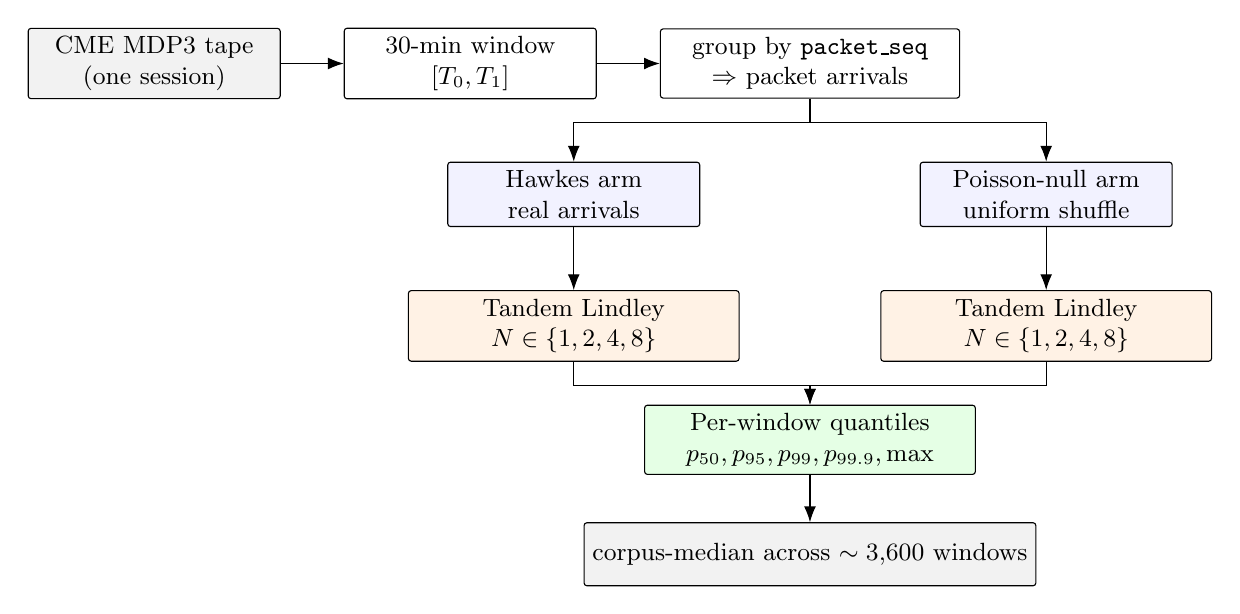
\begin{tikzpicture}[
    node distance=6mm and 8mm,
    box/.style={draw, rounded corners=1pt, align=center, minimum height=8mm, inner sep=3pt, font=\small},
    tape/.style={box, fill=black!5, minimum width=32mm},
    arm/.style={box, fill=blue!5, minimum width=32mm},
    sim/.style={box, fill=orange!10, minimum width=42mm},
    agg/.style={box, fill=green!10, minimum width=42mm},
    arrow/.style={-{Latex[length=2mm]}},
]
\node[tape] (tape) {CME MDP3 tape\\ (one session)};
\node[box, right=of tape, minimum width=32mm] (window) {30-min window\\ $[T_0, T_1]$};
\node[box, right=of window, minimum width=38mm] (packets) {group by \texttt{packet\_seq}\\ $\Rightarrow$ packet arrivals};

\node[arm, below=8mm of packets, xshift=-30mm] (hawkes) {Hawkes arm\\ real arrivals};
\node[arm, below=8mm of packets, xshift=+30mm] (poisson) {Poisson-null arm\\ uniform shuffle};

\node[sim, below=8mm of hawkes] (simH) {Tandem Lindley\\ $N \in \{1,2,4,8\}$};
\node[sim, below=8mm of poisson] (simP) {Tandem Lindley\\ $N \in \{1,2,4,8\}$};

\node[agg, below=10mm of $(simH)!0.5!(simP)$] (agg) {Per-window quantiles\\ $p_{50}, p_{95}, p_{99}, p_{99.9}, \max$};
\node[box, below=6mm of agg, minimum width=42mm, fill=gray!10] (corpus) {corpus-median across $\sim 3{,}600$ windows};

\draw[arrow] (tape) -- (window);
\draw[arrow] (window) -- (packets);
\draw[arrow] (packets.south) -- ++(0,-3mm) -| (hawkes.north);
\draw[arrow] (packets.south) -- ++(0,-3mm) -| (poisson.north);
\draw[arrow] (hawkes) -- (simH);
\draw[arrow] (poisson) -- (simP);
\draw[arrow] (simH.south) -- ++(0,-3mm) -| (agg.north);
\draw[arrow] (simP.south) -- ++(0,-3mm) -| (agg.north);
\draw[arrow] (agg) -- (corpus);
\end{tikzpicture}
\caption{Per-window data flow of the empirical experiment. A single session tape is chopped into 30-minute RTH windows. Each window's messages are grouped by \texttt{packet\_seq} into a real packet-arrival stream (Hawkes arm). A rate-matched Poisson-null arm is generated by uniformly shuffling the same arrival count over the same window. Both arms are run through the $N$-stage tandem Lindley simulator at $N \in \{1, 2, 4, 8\}$. Per-window quantiles are recorded and aggregated by corpus median across all $\sim 3{,}600$ windows in the 281-session corpus.}
\label{fig:experiment}
\end{figure}

\begin{algorithm}[H]
\caption{Per-window procedure of the empirical experiment.}
\label{alg:sweep}
\begin{algorithmic}[1]
\State \textbf{input:} session tape $S$, service $T$, hop $h$, stage counts $\mathcal{N}$
\For{each 30-min RTH window $W$ in $S$ with $[T_0, T_1]$}
    \State $\{m_i\} \gets$ messages in $W$
    \State $\{(\text{seq}, t)\} \gets \{(\text{packet\_seq}(m_i), \text{transactTime}(m_i))\}$
    \State $\text{arr}_H \gets \text{sort}\big(\{\min_i t_i : \text{seq}_i = s\}_s\big)$ \Comment{Hawkes arm (real arrivals)}
    \State $n_{\mathrm{pkt}}^{\#} \gets |\text{arr}_H|$
    \State $\text{arr}_P \gets \text{sort}\big(\text{Uniform}(T_0, T_1)^{n_{\mathrm{pkt}}^{\#}}\big)$ \Comment{Poisson-null arm (seeded per window)}
    \For{regime $\in \{H, P\}$, $N \in \mathcal{N}$}
        \State $\text{lat} \gets \textsc{TandemLindley}(\text{arr}_{\text{regime}}, N, T, h)$
        \State record $\big(S, W, \text{regime}, N, \{p_{50}, p_{95}, p_{99}, p_{99.9}, \max\}(\text{lat})\big)$
    \EndFor
\EndFor
\State \Return corpus-median of each recorded quantile across all $(S, W)$ pairs
\Function{TandemLindley}{$\text{arr}, N, T, h$}
    \State $\text{dep} \gets \text{arr}$
    \For{stage $k = 1, \ldots, N$}
        \If{$k > 1$} $\text{dep} \gets \text{dep} + h$ \EndIf
        \State $\text{dep} \gets \text{dep} + \textsc{Lindley}(\text{dep}, T/N)$
    \EndFor
    \State \Return $\text{dep} - \text{arr}$
\EndFunction
\end{algorithmic}
\end{algorithm}

\subsection{Data corpus}
\label{sec:setup-data}

The corpus is 281 sessions of CME MDP3 channel 318 (NQ) front-month pcap-derived tapes covering 2025-01 through 2026-02, RTH only, holidays and half-days excluded. Each MBO record carries a nanosecond \texttt{transactTime} (the CME matching-engine event time in the MDP3 message body) and a \texttt{packet\_seq} (the UDP packet sequence number). Messages are grouped into packets by \texttt{packet\_seq}; a packet's arrival time is the minimum \texttt{transactTime} of its constituent events. Each session tape is chopped into non-overlapping 30-minute RTH windows; for each window we compute the packet-arrival stream and the per-window quantities listed in Section~\ref{sec:notation}. The full corpus produces $\sim 3{,}600$ per-window records: 281 sessions $\times$ roughly 13 windows per RTH day.

% =====================================================================

\subsection{Packet arrivals are Hawkes-clustered (empirical prerequisite)}
\label{sec:setup-hawkes}

The paper's simulator input is the packet-arrival stream, so the first empirical question is whether that stream is clustered or Poisson. Three model-free and one model-based diagnostic on the 281-session NQ front-month corpus all reject Poisson decisively. The fraction of interarrival gaps shorter than one-tenth of the mean gap is 40--85\% per 30-minute window, versus the Poisson benchmark $1 - e^{-0.1} \approx 9.52\%$ that would obtain for any exponential-gap process regardless of rate. The Fano factor $F(T) = \mathrm{Var}[C_T] / \mathrm{E}[C_T]$ of packet counts in windows of length $T$ rises from $F(0.1\,\mathrm{s}) \approx 2$ to $F(60\,\mathrm{s}) \approx 40$ across the corpus median, versus $F(T) \equiv 1$ for Poisson at every $T$; the log-log fit gives a Hurst exponent $H \approx 0.65$--$0.75$, versus $H = 0.5$ for Poisson. Fitting the standard exponential-kernel Hawkes process $\lambda(t) = \mu + \sum_{t_i < t} \alpha\, e^{-\beta(t - t_i)}$ to each window by MLE (Ogata log-likelihood with the standard recursive intensity, closed-form compensator, Nelder--Mead over $(\mu, \alpha, \beta)$) gives a branching ratio $n = \alpha/\beta$ in the range $0.75$--$0.85$ across the windows processed so far (599 windows over 47 sessions; the full-corpus fit is in flight), with a corpus median of $0.79$ and every fit converged; the same optimum is recovered by a reparameterised L-BFGS-B fit to four decimals on spot-checked windows. This is the same near-critical regime that \citet{filimonovsornette2012} and \citet{hardimanbercotbouchaud2013} document on ES, at a somewhat lower level than their $n \approx 0.9$; they fit trade arrivals rather than packet arrivals, and a packet aggregates several book events, which is expected to lower the fitted self-excitation. Fisher--Yates shuffle of the interarrival gap sequence within each window destroys the clustering entirely --- shuffled Fano at $T = 5\,\mathrm{s}$ collapses to $\approx 1$ --- confirming that the excess variance lives in the ordering, not in the marginal gap distribution (i.e., Hawkes rather than a heavy-tailed renewal process). The paper's downstream simulator is therefore driven by an arrival process that is empirically far from Poisson, and any tail-latency finding based on a matched-rate Poisson null represents a hard counterfactual, not a straw man.

% =====================================================================

\subsection{Simulator}
\label{sec:setup-simulator}
\label{sec:sim-model}

Packet arrivals $t_1 < t_2 < \cdots$ enter stage 1. Each stage $k$ is a single-server FIFO queue with deterministic service $T/N$ (own actor, own thread), and departures from stage $k$ are delayed by $h$ before arriving at stage $k+1$. Standard Lindley recursion per stage:
\begin{equation}
W^{(k)}_{i+1} = \max\!\left(0,\; W^{(k)}_i + \frac{T}{N} - (a^{(k)}_{i+1} - a^{(k)}_i)\right),
\end{equation}
with $a^{(k+1)}_i = a^{(k)}_i + W^{(k)}_i + T/N + h$.

\subsection{Pipelining is what makes multi-stage work}
\label{sec:sim-pipeline}

The tandem is a \emph{pipelined} design: each stage's actor runs on its own thread, so at the same wall-clock instant stage 2 can be processing message $k-1$ while stage 1 is processing message $k$. The simulator captures this implicitly because Lindley is applied separately per stage and each stage tracks its own ``when did the previous message leave'' timeline --- the two servers' busy intervals overlap on the wall-clock axis.

Worked example. Three packets arriving at $t = 0, 1, 2\,\mu\mathrm{s}$; single-stage total service $T = 10\,\mu\mathrm{s}$; two-stage tandem with per-stage service $T/2 = 5\,\mu\mathrm{s}$ and hop $h = 1.7\,\mu\mathrm{s}$:

\begin{center}
\begin{tabular}{lrrr}
\toprule
 & msg 1 & msg 2 & msg 3 \\
\midrule
single-stage arrival & 0 & 1 & 2 \\
single-stage latency ($\mu$s) & 10.0 & 19.0 & \textbf{28.0} \\
\midrule
tandem arrive stage 1 & 0.0 & 1.0 & 2.0 \\
tandem wait stage 1 & 0.0 & 4.0 & 8.0 \\
tandem leave stage 1 & 5.0 & 10.0 & 15.0 \\
tandem arrive stage 2 ($+h$) & 6.7 & 11.7 & 16.7 \\
tandem wait stage 2 & 0.0 & 0.0 & 0.0 \\
tandem leave stage 2 & 11.7 & 16.7 & 21.7 \\
\textbf{tandem latency ($\mu$s)} & \textbf{11.7} & \textbf{15.7} & \textbf{19.7} \\
\bottomrule
\end{tabular}
\end{center}

At wall-clock $t \approx 7$, stage 1's actor is busy on message 2 while stage 2's actor is busy on message 1 --- two actors doing useful work at the same time. Message 1 pays a $1.7\,\mu\mathrm{s}$ hop cost (latency $10.0 \to 11.7$); message 3, at the burst tail, drops from $28.0$ to $19.7\,\mu\mathrm{s}$. Median hurts, tail wins --- same message count, throughput $2/T$ rather than $1/T$. This is exactly the mechanism of Theorem~\ref{thm:burst}.

\paragraph{Pipelining is a necessary condition, not a nice-to-have.} The tail-latency improvement in Theorem~\ref{thm:burst} and Theorem~\ref{thm:reduction} comes entirely from concurrent execution across the $N$ stages: at any wall-clock instant, several different messages are simultaneously in flight at different stages of the pipeline, and it is that overlap that raises system throughput from $1/T$ to $\min_i 1/s_i$ (equal to $N/T$ under equal-sized stages). Take away the concurrency --- for instance by chaining $N$ synchronous handoffs on a single thread, where the sender blocks until each downstream stage finishes --- and the entire benefit disappears. In that case each message serially traverses all $N$ stages before the next message can start; total service work per message is still $T$, so throughput remains $1/T$, and the pipeline adds $(N-1)h$ of hop cost with no compensating tail win. Under Hawkes bursts a synchronous $N$-stage chain is strictly worse than a single-stage event loop by exactly $(N-1)h$ per message. Pipelining --- concurrent execution of different messages at different stages on different threads --- is therefore not an optimisation on top of the tandem design, it is the design; the paper's simulator captures this by applying Lindley separately per stage, giving each stage its own busy-idle timeline. The framework-implementation Section~\ref{sec:implementation} discusses which \kasparhft{} dispatch paths actually deliver this concurrency (the asynchronous BQueue path) and which do not (the synchronous \texttt{fast\_send} path, which despite its low per-call cost does not support pipelining).

\paragraph{Calibration and cost.} The paper reports numerical results at $h = 1.7\,\mu\mathrm{s}$ --- the one-way async mailbox cost obtained by halving the round-trip figure in Table~4 of \citet{mayeski_fastsend} and consistent with the shipping \kasparhft{} BQueue path characterised in \citet{mayeski_actorhft} --- swept across $T \in \{2, 4, 8, 16, 32\}\,\mu\mathrm{s}$ to cover the sub-hop regime through the slow-servicing regime. The simulator is deterministic given the tape and $(T, h, N)$; one $O(n)$ pass per stage per window makes its wall-clock cost negligible next to the tape read.

% =====================================================================

\subsection{Sweep design}
\label{sec:setup-sweep}

The design asks whether an $N$-stage tandem reduces $p_{99}$ latency under real Hawkes packet arrivals and whether the same architecture achieves the same compression under a rate-matched Poisson null. For each 30-minute window we run the tandem Lindley of Section~\ref{sec:setup-simulator} at $N \in \{1, 2, 4, 8\}$ under two arrival regimes: the real packet-arrival timestamps from the tape (Hawkes arm) and a uniform-shuffle of the same $n_{\mathrm{pkt}}^{\#}$ arrivals into the same window (Poisson-null arm; equivalent to a homogeneous Poisson process at rate $n_{\mathrm{pkt}}^{\#} / (T_1 - T_0)$ conditional on the count). Per (window, $N$, regime) we record $p_{50}, p_{95}, p_{99}, p_{99.9}, \max$ of end-to-end latency. Aggregation is corpus-median across all windows; the two headline curves per scenario are $p_{99}(N)$ and $p_{50}(N)$ under Hawkes and Poisson overlaid.

The paper's empirical calibration is $h = 1.7\,\mu\mathrm{s}$ (one-way async cross-thread mailbox cost, per \citet{mayeski_fastsend}'s Table~4 halved for one-way) swept over $T \in \{2, 4, 8, 16, 32\}\,\mu\mathrm{s}$ so the scenarios span from the sub-hop regime through the slow-servicing regime. Theorem~\ref{thm:reduction} predicts $p_{99}^{\mathrm{H}}(N) - (N-1)h - T \le \big(p_{99}^{\mathrm{H}}(1) - T\big)/N$ on every window, i.e.\ a fitted exponent $\gamma \ge 1$ in $\Delta(N) \approx \Delta(1) N^{-\gamma}$; Corollary~\ref{cor:poisson} predicts $p_{99}^{\mathrm{P}}(N) = p_{50}^{\mathrm{P}}(N) = T + (N-1)h$ exactly; any of (i) a window on which the Hawkes bound is violated, (ii) Poisson $p_{99}(N)$ exceeding $T + (N-1)h$, or (iii) Hawkes $p_{50}(N)$ growing at slope $\gg h$ per stage falsifies the paper's model of the simulator.

% =====================================================================

\section{Empirical results}
\label{sec:results}

\emph{Data-refresh note.} The numbers in this section are from an earlier interim run at $T \in \{10, 20\}\,\mu\mathrm{s}$ and $h = 3\,\mu\mathrm{s}$, retained here to show the qualitative shape of the tail collapse. The paper's canonical sweep --- $T \in \{2, 4, 8, 16, 32\}\,\mu\mathrm{s}$ at the corrected one-way hop cost $h = 1.7\,\mu\mathrm{s}$ --- is running on the full 281-session corpus and will replace the numbers below in the final revision; the qualitative claims (Hawkes tail collapse under splitting, Poisson null loss, median linear in $(N-1)h$) are not expected to change.

\subsection{Tail collapse under Hawkes, not under Poisson}
\label{sec:results-tail}

Table~\ref{tab:main-corpus} reports corpus-median $p_{50}$ and $p_{99}$ of end-to-end latency at the paper's main calibration point $T = 10\,\mu\mathrm{s}, h = 3\,\mu\mathrm{s}$: a typical HFT task under a wait/notify-scale async mailbox hop. Numbers come from a 23-session / 287-window interim run of \texttt{qsim\_grid.py}; the full 281-session batch is running and the final version will refresh the tables.

\begin{table}[H]
\centering
\begin{tabular}{@{}rrrrr@{}}
\toprule
$N$ & Hawkes $p_{50}$ (\si{\micro\second}) & Hawkes $p_{99}$ (\si{\micro\second}) & Poisson $p_{50}$ (\si{\micro\second}) & Poisson $p_{99}$ (\si{\micro\second}) \\
\midrule
1  & 10.00 & \textbf{39.96} & 10.00 & 10.00 \\
2  & 13.00 & \textbf{22.66} & 13.00 & 13.00 \\
4  & 19.00 & 22.39 & 19.00 & 19.00 \\
8  & 31.00 & 32.25 & 31.00 & 31.00 \\
\bottomrule
\end{tabular}
\caption{Corpus-median latency quantiles at $T = 10\,\mu\mathrm{s}, h = 3\,\mu\mathrm{s}$. 23 sessions, 287 30-minute windows (interim). Hawkes = real CME MDP3 NQ front-month packet arrivals; Poisson = uniform-shuffle null with the same arrival count per window.}
\label{tab:main-corpus}
\end{table}

Under Poisson the queue is essentially always empty at realistic CME utilisation, so every quantile equals the service floor exactly: $p_{50} = p_{99} = T + (N-1)h$. The Poisson counterfactual has no tail at all --- splitting under Poisson strictly loses.

Under Hawkes the story is completely different. Single-stage $p_{99}$ is $39.96\,\mu\mathrm{s}$ --- $4.0\times$ the service floor, entirely a clustering artefact. Splitting into $N = 2$ (two $5\,\mu\mathrm{s}$ tasks with one $3\,\mu\mathrm{s}$ hop) drops Hawkes $p_{99}$ to $22.66\,\mu\mathrm{s}$ --- a $17.3\,\mu\mathrm{s}$ tail-win at a $3\,\mu\mathrm{s}$ median cost. $N = 4$ is marginally lower still ($22.39\,\mu\mathrm{s}$, a difference inside the window-to-window noise), and $N = 8$ loses the tail win back to the accumulating hop cost. By $p_{99}$ alone the minimum sits at $N = 4$; by the design equation of Section~\ref{sec:results-design}, which also charges the median, $N^\star = 2$ for any tail weight $\kappa \le 0.96$. Either way two stages beat one on the tail by a wide margin, and $N = 8$ overshoots.

\subsection{Median cost is linear in $N$, exactly as $(N-1)h$}
\label{sec:results-median}

The $p_{50}$ column in Table~\ref{tab:main-corpus} matches Theorem~\ref{thm:burst}'s single-message formula:
\[
p_{50}^{\mathrm{H}}(N) = T + (N-1) h \pm \epsilon \quad \text{with}\quad T = 10, h = 3.
\]
Predicted 10, 13, 19, 31; measured 10.00, 13.00, 19.00, 31.00. Exact at all $N$. Under Poisson the identity is exact because the queue is always empty. Under Hawkes the identity holds because $p_{50}$ sits inside quiet inter-cluster stretches where the queue is also empty.

\subsection{Design equation}
\label{sec:results-design}

From the corpus fit:
\begin{align}
p_{99}^{\mathrm{Hawkes}}(N) &\;\approx\; T + (N-1)h + \Delta(N), \label{eq:design99} \\
p_{50}^{\mathrm{Hawkes}}(N) &\;\approx\; T + (N-1)h, \label{eq:design50}
\end{align}
where $\Delta(N) \equiv p_{99}^{\mathrm{Hawkes}}(N) - p_{50}^{\mathrm{Hawkes}}(N)$ is the ``clustering tail excess.'' On the 23-session interim run at $T=10, h=3$:
\[
\Delta(1) = 29.96, \quad \Delta(2) = 9.66, \quad \Delta(4) = 3.39, \quad \Delta(8) = 1.25\,\mu\mathrm{s}.
\]
A least-squares log-log fit gives $\Delta(N) \approx \Delta(1)\,N^{-\gamma}$ with $\gamma \approx 1.5$ on the interim data ($1.53$ at $T = 10$, $1.64$ at $T = 20$). Theorem~\ref{thm:reduction} guarantees $\gamma \ge 1$, with equality on isolated bursts; the excess $\gamma - 1 \approx 0.5$ is the slack in Equation~\eqref{eq:bound}, which arises because the tandem's bottleneck stage runs at utilisation $\rho/N$ and drains inter-cluster idle gaps $N$ times faster in absolute time than the single stage. The same excess appears in the synthetic check of Appendix~\ref{app:check}.

The operator's stage-count optimum is
\[
N^\star \;=\; \arg\min_N \Big[ (N-1) h \;+\; \kappa \, \Delta(N) \Big]
\]
for the operator's risk-aversion coefficient $\kappa$. Numerically at $T = 10, h = 3$ over the simulated grid $N \in \{1, 2, 4, 8\}$: $N^\star = 1$ for $\kappa < 0.15$, $N^\star = 2$ for $\kappa \in [0.15, 0.96]$, $N^\star = 4$ for $\kappa \in (0.96, 5.6]$, and $N^\star = 8$ only for $\kappa > 5.6$; the total end-to-end $p_{99}$ itself starts increasing beyond $N = 4$ because the accumulated $(N-1)h$ overtakes the residual $\Delta(N)$.

At real cut points the stages are unequal, and by Remark~\ref{rem:unequal} the tail excess depends on the partition $P$ of the servicing chain only through its largest stage, $\Delta(P) = \Delta_{\mathrm{single}}(s_{\max}(P))$, i.e.\ the single-stage tail excess measured at service $s_{\max}$. The optimum over partitions is then
\[
P^\star \;=\; \arg\min_P \Big[ \mathrm{hops}(P)\, h \;+\; \kappa\, \Delta_{\mathrm{single}}\big(s_{\max}(P)\big) \Big],
\]
which the interim tables let the operator evaluate directly: $\Delta_{\mathrm{single}}(s)$ at $s = 10, 5, 2.5, 1.25\,\mu\mathrm{s}$ is the $N = 1$ column of Table~\ref{tab:main-corpus} and the diagonal of Table~\ref{tab:scenarios}. Two rules of thumb fall out. A cut is worth its hop only if it lowers $s_{\max}$ by enough that $\kappa\,[\Delta_{\mathrm{single}}(s_{\max}) - \Delta_{\mathrm{single}}(s_{\max}')] > h$; and among partitions with the same $s_{\max}$ the one with the fewest hops wins outright, so sub-tasks downstream of the bottleneck should be merged onto one thread until their sum reaches $s_{\max}$.

\paragraph{Floor on $T$: short tasks cannot be usefully split.} Equations~\eqref{eq:design99}--\eqref{eq:design50} carry an obvious lower bound on the tasks the paper's recommendation applies to. The per-stage service is $T/N$, so splitting a task of total service $T$ into $N$ stages spends $(N-1) h$ of median cost to obtain the compression of a tail excess $\Delta(N)$ that itself cannot exceed the service floor $T$ by more than a constant multiplier set by the arrival law. When $T$ is of order the hop cost $h$ or below, the median cost per additional stage $h$ is already comparable to the entire single-stage latency $T$, and no achievable $\Delta(N)$ tail-win can offset it: the design equation prescribes $N^\star = 1$ mechanically. Concretely at the paper's calibration $h = 1.7\,\mu\mathrm{s}$, a task with $T = 1\,\mu\mathrm{s}$ cannot be usefully split into two half-microsecond stages --- one hop alone would add $1.7\,\mu\mathrm{s}$ of median to a task that clears in $1\,\mu\mathrm{s}$, for a tail-win bounded above by roughly $T$ itself; the $T = 2\,\mu\mathrm{s}$ row of the paper's sweep is included precisely to demonstrate that floor empirically. The ``prefer to split long tasks'' rule presupposes $T$ above the $2h$ floor; on this framework's shipping BQueue path ($h \approx 1.7\,\mu\mathrm{s}$) that floor is $T \gtrsim 3.4\,\mu\mathrm{s}$. The paper's $T = 2\,\mu\mathrm{s}$ row therefore sits below the floor ($\sim 41\%$ below) and is included as a demonstration case; $T = 4\,\mu\mathrm{s}$ sits only $\sim 18\%$ above and is an edge case where the design equation is barely applicable; $T \in \{8, 16, 32\}\,\mu\mathrm{s}$ sit comfortably above the floor and are the regime where the rule reliably applies. Sub-microsecond tasks --- for instance a single SBE integer decode, or a small handler that fires from a strategy fast path --- belong on \texttt{fast\_send}, not on a cross-thread mailbox, regardless of feed statistics.

\subsection{Comparison scenario: $T = 20\,\mu\mathrm{s}$}
\label{sec:results-scenarios}

Table~\ref{tab:scenarios} reports the same sweep for a slower task, $T = 20\,\mu\mathrm{s}$ at the same $h = 3\,\mu\mathrm{s}$.

\begin{table}[H]
\centering
\begin{tabular}{@{}rrrrr@{}}
\toprule
$N$ & Hawkes $p_{50}$ (\si{\micro\second}) & Hawkes $p_{99}$ (\si{\micro\second}) & Poisson $p_{50}$ (\si{\micro\second}) & Poisson $p_{99}$ (\si{\micro\second}) \\
\midrule
1  & 20.00 & \textbf{121.74} & 20.00 & 20.00 \\
2  & 23.00 & \phantom{0}52.96 & 23.00 & 23.00 \\
4  & 29.00 & \textbf{38.66}   & 29.00 & 29.00 \\
8  & 41.00 & \phantom{0}44.39 & 41.00 & 41.00 \\
\bottomrule
\end{tabular}
\caption{Corpus-median latency quantiles at $T = 20\,\mu\mathrm{s}, h = 3\,\mu\mathrm{s}$. 23 sessions, 287 30-minute windows (interim).}
\label{tab:scenarios}
\end{table}

At $T = 20\,\mu\mathrm{s}$ the single-stage Hawkes $p_{99}$ is $121.7\,\mu\mathrm{s}$ --- a $6.1\times$ multiplier over the service floor, larger than the $4.0\times$ at $T = 10$ because burst-clearing time scales with $T$. The tail-win compounds: $N = 2$ gives $-69\,\mu\mathrm{s}$, $N = 4$ gives $-83\,\mu\mathrm{s}$, before $N = 8$ starts losing it back. Optimum is $N^\star = 4$ under $T = 20$. Under Poisson the tail wins are zero and the median cost is real at every $N$, exactly as Corollary~\ref{cor:poisson} predicts.

\subsection{Sensitivity to $h$}
\label{sec:results-h}

The design equation is monotone in $h$: at fixed $T$ and fixed corpus $\Delta(N)$, the operator's $N^\star$ shrinks as $h$ grows. At $h = 1.7\,\mu\mathrm{s}$ (this paper's calibration) the design equation predicts $N^\star = 1$ at $T = 2\,\mu\mathrm{s}$ (below the $2h$ floor), and $N^\star \geq 2$ for $T \gtrsim 4\,\mu\mathrm{s}$ conditional on the corpus $\Delta(N)$; the exact $N^\star$ per row of the sweep, including whether it plateaus or increases monotonically with $T$, will be reported when the full sweep completes. At lower $h$ (a hypothetical busy-poll async mailbox in the sub-microsecond regime), $N^\star$ climbs faster toward the natural cut-point ceiling of $4$--$5$.

\paragraph{$h$ is load-dependent; $1.7\,\mu\mathrm{s}$ is a conservative upper bound.} The $h = 1.7\,\mu\mathrm{s}$ figure is the one-way cost of the shipping \kasparhft{} BQueue mailbox measured at low load, where the receiver is sleeping on a condition variable and the send path must pay the kernel wake latency to bring it back onto CPU. That wake latency is the dominant term in the $\sim\!3.4\,\mu\mathrm{s}$ round-trip of Table~4 in \citet{mayeski_fastsend}, and the general fact that a spinning receiver delivers a message an order of magnitude faster than a wake-from-condvar receiver is standard in the microsecond-latency systems literature: \citet{david2013synch} measure the primitive costs directly on commodity Linux hardware, \citet{belay2014ix} exploit this in the IX data plane by pinning busy-polling network threads, and Rigtorp's operational guide \citep{rigtorp_lowlatency} formalises the ``run one thread per core and busy-wait'' rule that flows from it; the fast\_send paper's own grouped-\texttt{send} row (Table~4, $\sim\!90$ ns) is the same effect on the same framework --- when the receiver never actually sleeps, the send path collapses. Under sustained load, and specifically inside a Hawkes cluster where the receiver's queue is never empty, the receiver never sleeps: successive messages arrive faster than the receiver's per-message service time, so it stays awake in a tight run-loop and the enqueue path reduces to a mutex acquire, a queue push, and a condition-variable notify against a receiver that is not waiting (a near-no-op). The effective $h$ in that regime is dominated by the mutex $+$ cache-line-transfer cost, typically a few hundred nanoseconds rather than $1.7\,\mu\mathrm{s}$. This is exactly the operating regime in which the paper's tail-latency win is largest --- the win compounds while $h$ shrinks --- so the paper's reported effect underestimates the true benefit whenever the pipeline is inside a burst. Characterising the load-conditioned hop cost $h(\rho)$ is left to future work; a full accounting would strengthen the results reported here.



% =====================================================================

% =====================================================================

\clearpage
\part{Evaluation and implementation}

\section{Evaluation: do empirics match the analytical predictions?}
\label{sec:evaluation}

This section compares the empirical numbers of Section~\ref{sec:results} against the closed-form predictions of Section~\ref{sec:theory}.

\paragraph{Theorem~\ref{thm:burst} (burst-limit throughput).} The single-message identity $p_{50}^{\mathrm{H}}(N) = T + (N-1) h$ is predicted exactly by Theorem~\ref{thm:burst} for any arrival law when $p_{50}$ falls in a quiet inter-cluster stretch (queue empty). The interim $T = 10, h = 3\,\mu\mathrm{s}$ run confirms this identity exactly for every $N \in \{2, 4, 8\}$ in Table~\ref{tab:main-corpus} (per-stage service $T/N$ divides evenly at these values). The $h = 1.7\,\mu\mathrm{s}$ sweep now in flight is expected to reproduce the identity across the same $N$ range against the new hop calibration.

\paragraph{Theorem~\ref{thm:reduction} (reduction and scaling bound).} The prediction is $\Delta(N) \le \Delta(1)/N$ on every window, i.e.\ $\gamma \ge 1$. On the interim $h = 3\,\mu\mathrm{s}$ run the corpus-median tail excess ratios $\Delta(N)/\Delta(1)$ at $T = 10$ were $0.32, 0.11, 0.04$ for $N = 2, 4, 8$ against bounds of $0.50, 0.25, 0.125$; at $T = 20$ they were $0.29, 0.09, 0.03$. The bound holds at every $(T, N)$ with the slack expected from the $\rho/N$ utilisation effect. The reduction identity Equation~\eqref{eq:reduction} is also visible directly in the interim tables: the tail excess $\Delta$ depends on $(T, N)$ only through $s_{\max} = T/N$, so it should coincide along diagonals of constant $T/N$, and it does to the reported precision, $\Delta(T{=}20, N{=}2) = \Delta(T{=}10, N{=}1) = 29.96$, $\Delta(20, 4) = \Delta(10, 2) = 9.66$, $\Delta(20, 8) = \Delta(10, 4) = 3.39\,\mu\mathrm{s}$ (Tables~\ref{tab:main-corpus} and~\ref{tab:scenarios}). The bound is pathwise, so it should hold on every individual window and at every quantile, and the $h = 1.7\,\mu\mathrm{s}$ sweep will report the per-window violation count (expected to be zero, up to the simulator's discretisation of $T/N$) alongside the fitted $\gamma$ across the full $T \in \{2, 4, 8, 16, 32\}\,\mu\mathrm{s}, N \in \{1, 2, 4, 8\}$ grid.

\paragraph{Corollary~\ref{cor:poisson} (Poisson null).} The prediction is $p_{99}^{\mathrm{P}}(N) = p_{50}^{\mathrm{P}}(N) = T + (N-1)h$ under matched-rate Poisson arrivals at the corpus utilisation: the single-stage wait is already zero, so splitting costs exactly the hops. On the interim run at both $T = 10$ and $T = 20$, Poisson $p_{99}$ equalled Poisson $p_{50}$ at every $N$, and both grew exactly as $T + (N-1)h$: the corollary matches on the nose. The $h = 1.7\,\mu\mathrm{s}$ sweep is expected to reproduce this exactly, and its $p_{99.9}$ column will show whether the Poisson wait first becomes visible at that quantile, as $\Pr(W^{(1)} > 0) = \rho$ predicts once $\rho$ exceeds $10^{-3}$.

\paragraph{Verdict.} All three analytical statements survive their empirical test on the interim run. The quantitatively load-bearing one, $\gamma \ge 1$, holds with room to spare, and the full corpus sweep will produce a fitted $\gamma$ and a per-window bound check on all 281 sessions.

\section{Implementing a multi-actor pipeline}
\label{sec:implementation}

The design equation maps onto framework choices in a specific way. The paper's model of an $N$-stage tandem assumes each stage's actor runs on its own thread and sends its output to the next stage through an asynchronous mailbox --- that is what makes the pipeline pipelined, and the hop cost $h$ is the wall-clock latency of that asynchronous handoff.

\paragraph{Two hop paths in the shipping \kasparhft{} framework.} \kasparhft{} is a shared-nothing C++20 actor framework with two distinct dispatch paths that this paper needs to distinguish. Actors register under a \texttt{Manager}, groups of actors sharing a thread register as \texttt{Group}s, and messages flow one-way with no shared state. The default asynchronous send uses \texttt{BQueue}, a blocking mailbox built on \texttt{std::mutex} $+$ \texttt{std::condition\_variable} $+$ \texttt{boost::circular\_buffer}; a producer thread enqueues under the mutex and a consumer thread waits on the condition variable. This is the hop path the paper's Section~\ref{sec:setup-simulator} model corresponds to. \citet{mayeski_fastsend} Table~4 measures the round-trip cost of a cross-thread \texttt{send} at $\sim 3.4\,\mu\mathrm{s}$; the pipeline's one-way hop cost is therefore $h \approx 1.7\,\mu\mathrm{s}$ for a real pipelined tandem built on \kasparhft{}'s current mailbox.

The \texttt{fast\_send} path is different: it is a \emph{synchronous} dispatch that acquires a per-actor mutex, calls the receiver's handler inline on the sender's thread, and returns the reply. There is no queue and no cross-thread wake-up. Its per-call cost is much smaller than the BQueue path's, but it is not a pipelined hop: the sender blocks until the receiver finishes, so a chain of \texttt{fast\_send}s serialises through all stages on one thread and offers none of the throughput speedup of Theorem~\ref{thm:burst}. The paper's design equation does not apply to \texttt{fast\_send} chains.

The two dispatch paths present a critical property that Section~\ref{sec:fungibility} discusses in detail: they are \emph{fungible} at the sender's call site with no receiver-side change. That fungibility is what makes the design equation's recommendation actionable as an end-of-build optimization rather than an early-stage architecture commitment.

\paragraph{Natural cut points on a CME MDP3 handler.} The decode pipeline decomposes into four to five actors: \texttt{SocketReader} (UDP reception), \texttt{MessageProcessor} / SBE decoder, order-book actor (MBP or MBO), strategy actor (\shadowpov{} in \kasparhft{}), order manager. These are the paper's cut points; $N > 5$ requires artificial decomposition and hits diminishing returns.

\paragraph{Applying the design equation.} At the paper's calibration $h = 1.7\,\mu\mathrm{s}$ (matching the shipping \kasparhft{} BQueue path per \citet{mayeski_fastsend}~Table~4 halved for one-way), Section~\ref{sec:results-design}'s design equation recommends splitting whenever $T$ is comfortably above $\sim 3.4\,\mu\mathrm{s}$. The interim $T = 10\,\mu\mathrm{s}, h = 3\,\mu\mathrm{s}$ run gave $N^\star = 2$ for tail weights up to $\kappa \approx 1$ and $N^\star = 4$ above, at a small median cost for a large tail-win under Hawkes arrivals; the sweep now in flight will refine those values at the corrected $h$. Larger $N$ eventually costs more on the median than it recovers on the tail once $(N-1)h$ approaches the remaining clustering tail excess. A sub-microsecond $h$ obtained via a busy-poll async mailbox would raise the recommended $N$ toward the natural cut-point ceiling of four or five --- but Section~\ref{sec:other-arch} argues that on a Hawkes feed the receiver is already effectively spinning during every $p_{99}$ arrival, so the practical ROI of a busy-poll upgrade over the shipping BQueue path is expected to be smaller than the standard low-latency-systems argument would suggest. That trade is a candidate follow-on measurement.

\paragraph{Operator-side hardening.} Beyond the framework's async-mailbox choice, further reductions of $h$ live in Linux configuration: actor-to-core pinning under \texttt{isolcpus}, NIC and timer IRQs steered off actor cores via \texttt{smp\_affinity}, real-time scheduling class \texttt{SCHED\_FIFO} on actor threads, huge pages. Kernel-bypass NIC data planes (Solarflare Onload, DPDK, VMA) help the exchange-to-decoder wire path but not the actor-to-actor hop, where both endpoints are already in userspace on the same host.

\paragraph{Falsification path for other frameworks.} If a framework's measured $h$ exceeds $T/N^\star$ for the operator's target $N^\star$, the design equation recommends against pipelining --- the median cost of a stage eats the tail win. The paper's recommendation is framework-specific: measure $h$ on your own dispatch path, plug it into Equation~\eqref{eq:design99}, and read off $N^\star$.

\paragraph{Cache pollution on spinning receivers.} A busy-poll receiver eliminates wake-up cost but pollutes L1/L2 caches on its host core and steals memory bandwidth. How many stages can be spun before the aggregate cache-pollution cost exceeds the tail-latency win is left to future work; the author's production experience with pinned busy-poll across a full servicing chain has been negative (Section~\ref{sec:other-arch}), which is one reason the paper's calibration uses the wait/notify mailbox rather than a spinning one.

% =====================================================================

\section{Fungibility of sync and async delivery in \kasparhft{}}
\label{sec:fungibility}

The central practical claim of this paper is that on Hawkes-clustered feeds the choice of \texttt{fast\_send} versus asynchronous \texttt{send} at each actor boundary is not an early-stage architectural commitment but a late-stage optimization decision --- one that should be made per boundary on the basis of measured end-to-end median and tail latency of the assembled pipeline against the target feed, not on the basis of local reasoning at any single call site. \kasparhft{} was designed to support this workflow. This section states the property that makes it possible, argues why it is critical from a system-optimization standpoint, and gives the operational discipline it enables.

\subsection{Receiver transparency}
\label{sec:fungibility-transparency}

Every actor in \kasparhft{} registers its handlers through the \texttt{MESSAGE\_HANDLER(MsgType,\ handler\_method)} macro. A handler is a function of one message argument; nothing in its body can access, observe, or condition on the delivery mode by which it was invoked. This property is called \emph{receiver transparency} in \citet{mayeski_fastsend} and is what makes the send-mode choice a purely sender-side decision.

Concretely:
\begin{itemize}
  \item \textbf{Synchronous delivery:} \texttt{target->fast\_send(m,\ this)}. The sender's thread acquires \texttt{target}'s per-actor mutex, calls the receiver's handler inline on the sender's thread, and takes the reply as a return value. No queue, no cross-thread wake-up. Round-trip cost $\sim 30$ ns per Table~4 of \citet{mayeski_fastsend}.
  \item \textbf{Asynchronous delivery:} \texttt{target->send(m,\ this)}. The message is enqueued on \texttt{target}'s BQueue mailbox (\texttt{mutex} $+$ \texttt{condition\_variable} $+$ \texttt{boost::circular\_buffer}); \texttt{target}'s own thread wakes up on the condition variable and runs the handler. Round-trip cost $\sim 3.4\,\mu\mathrm{s}$ across threads, or $\sim 90$ ns same-thread within a \texttt{Group}, per the same reference.
\end{itemize}
Both paths deliver the same handler with the same message. Neither the handler's body nor any actor downstream of it can tell which path fired. Switching a boundary between the two is a one-line change at the sender's call site --- \texttt{target->fast\_send(m,\ this)} $\leftrightarrow$ \texttt{target->send(m,\ this)} --- with no code change on the receiver side, no header change, no interface change, no test change.

\subsection{Why measurement, not local reasoning, must decide}
\label{sec:fungibility-why-measure}

The end-to-end latency profile of an HFT pipeline is a joint property of (i)~which stages exist and where they are cut, (ii)~which pairs of adjacent stages are joined by \texttt{fast\_send} versus \texttt{send}, and (iii)~the arrival law of the input feed. Theorem~\ref{thm:burst} and Theorem~\ref{thm:reduction} both fold across multiple boundaries: the throughput speedup is $N$-fold and the tail contraction is $N^{-\gamma}$ with $\gamma \ge 1$, so the joint optimum is emphatically not deducible from local reasoning at any single boundary. A designer who reasons at one boundary at a time --- "this hop is $\sim 1.7\,\mu\mathrm{s}$, that is a lot, use \texttt{fast\_send}" --- systematically underestimates the aggregate tail benefit of adding hops, and this is exactly the class of local reasoning that led the low-latency-systems community into the single-thread orthodoxy of Section~\ref{sec:intro-singlethread-priors}.

Getting the joint optimum therefore requires end-to-end measurement of the assembled pipeline against a representative feed, and iteration over per-boundary flips. The observable objective is a two-tuple $(p_{50}, p_{99})$ of end-to-end latency under the target feed, with an operator-chosen tradeoff between the two (Section~\ref{sec:results-design}'s $\kappa$). The design equation of Part~II supplies a first-principles prior on where the optimum sits under a Hawkes feed, but the measurement is the arbiter, not the equation.

\subsection{Operational discipline}
\label{sec:fungibility-workflow}

The \kasparhft{} design flow that this suggests, and which we now recommend as canonical for HFT actor pipelines running on self-exciting feeds, is:
\begin{enumerate}
  \item Draft the pipeline as a chain of actors at the natural cut points of the servicing chain (SBE decode, order book, strategy, order manager on CME MDP3; four to five stages per Section~\ref{sec:implementation}).
  \item Wire every intra-servicing-chain boundary with whichever of \texttt{fast\_send} or \texttt{send} is convenient during development; do not commit to a topology at this stage.
  \item Once the pipeline runs end-to-end on the target feed, measure the corpus-median $p_{50}$ and $p_{99}$ of end-to-end latency under the operator's live-representative tape, and record them as the baseline.
  \item Perturb one boundary at a time --- flip its \texttt{fast\_send} $\leftrightarrow$ \texttt{send} --- and re-measure. Accept the flip if $(p_{50}, p_{99})$ improves under the operator's chosen tradeoff.
  \item Iterate until no single-boundary flip improves the objective.
\end{enumerate}

Under the arrival law of a CME MDP3 feed the design equation of Section~\ref{sec:results-design} predicts what steps 4--5 converge to: async \texttt{send} at every boundary whose removal would raise the largest stage, and \texttt{fast\_send} everywhere else, in particular between short sub-tasks below the $2h$ floor of Section~\ref{sec:results-design} and between sub-tasks downstream of the bottleneck whose combined service stays at or below $s_{\max}$ (Remark~\ref{rem:unequal}). The operator does not need to trust that prediction to run the discipline; the measurement is the arbiter, and the arrival-law prior tells the operator where to expect it to land.

\subsection{Separation of code construction from latency optimization}
\label{sec:fungibility-decoupling}

A consequence of Section~\ref{sec:fungibility-workflow} that deserves separate emphasis: in \kasparhft{} \emph{two} distinct topology decisions are not knowable at design time. The first is the \emph{actor-to-thread mapping} --- which actors share a thread by being placed in a common \texttt{Group}, and which run on their own thread. The second is the \emph{per-boundary send-mode choice} --- whether each pair of adjacent actors is joined by synchronous \texttt{fast\_send} or asynchronous \texttt{send}. Neither decision is deducible from the source code alone. Both are functions of the target feed's arrival statistics and the operator's median-versus-tail tradeoff, both of which are properties of the deployment environment. The optimum can only be measured from the assembled system running against a representative feed.

Under receiver transparency this is a feature rather than a limitation. Actor code, message-type headers, and the full suite of unit and integration tests can be written and run before either the actor-to-thread mapping or the send-mode choice has been decided. Code construction and testing therefore proceed independently of the latency-optimization consideration --- both decisions are deferred to the end of the build, informed by measurements that could not have been taken any earlier because the system did not yet exist to measure. Correctness is established first; latency is optimized against the specific feed the system will run on, second. Two developers building two actors on the two sides of a boundary do not need to agree on whether their actors will ultimately live on the same thread or on different threads, nor on whether their handoff will be synchronous or asynchronous; they need to agree only on the message type. The message-type agreement is checkable at compile time; the two topology decisions are scalar dials adjusted at deployment.

This decoupling of correctness-phase engineering from latency-phase engineering is the practical payoff of receiver transparency, and it is what makes \kasparhft{}'s design cycle qualitatively different from frameworks in which either topology decision leaks into the receiver's interface (Section~\ref{sec:fungibility-contrast}). Design proceeds without a commitment to a topology; the commitment is made once, near deployment, on the basis of measurements the code did not need to know about while it was being written.

\subsection{Contrast with non-fungible frameworks}
\label{sec:fungibility-contrast}

Most low-latency actor frameworks bake the sender's choice of delivery mode into the receiver's type. An Akka actor's \texttt{tell} versus \texttt{ask}, a CAF actor's \texttt{send} versus \texttt{request}, and an Erlang process's cast versus call each expose different receiver-side surfaces, so flipping a boundary from sync to async is a small refactor rather than a one-line change. Under those frameworks the design flow of Section~\ref{sec:fungibility-workflow} is not tractable, and the operator's incentive is therefore to lock in the send-mode choice early --- reasoning locally --- rather than to defer it to an end-of-build measurement pass. This structural incentive is a plausible contributing cause of the single-thread orthodoxy: frameworks that penalise deferral push designers toward the topology that is least sensitive to a wrong early guess, which is the collapsed single-thread servicing chain.

\kasparhft{}'s joint mailbox API of \texttt{fast\_send} and \texttt{send}, and the receiver-transparency property underneath, are the concrete machinery that make measurement-driven send-mode optimization practical. That is the framework property this paper's design rule depends on operationally, and it is why we regard it as critical to system-level optimization on Hawkes-clustered feeds.

% =====================================================================

\section{Other architectural considerations to re-evaluate under Hawkes}
\label{sec:other-arch}

The paper's central claim is that the single-thread hot-path recommendation, treated as received wisdom in HFT infrastructure for over a decade, becomes wrong once the arrival law is recognised as Hawkes-clustered rather than Poisson (Section~\ref{sec:intro-singlethread-priors}, Section~\ref{sec:results}). Two adjacent architectural conventions in the same low-latency-systems canon --- pre-spinning receivers and pre-warming pipelines --- rest on the same implicit Poisson-load assumption, and this section flags them as deserving the same treatment. We do not measure either intervention here; both belong to future work. What follows is an argument that the arrival law itself provides most of the benefit these interventions are engineered to deliver, on the specific quantile that HFT operators care about.

\paragraph{Pre-spinning receivers.} The busy-poll recommendation of \citet{rigtorp_lowlatency}, \citet{belay2014ix}, and the Aeron/Chronicle lineage (Section~\ref{sec:intro-singlethread-priors}) pins a spinning thread per receiver so the wake path from a sleeping condition variable is never taken. On a Poisson feed, any arrival can find the receiver asleep, and the wake latency is paid on average; pre-spinning eliminates it. On a Hawkes feed with branching ratio $n \approx 0.8$, sleep/wake transitions happen only at cluster boundaries. Every $p_{99}$ message is intra-cluster (Section~\ref{sec:results-tail}: the $p_{99}$ message waits behind a cluster, since under the Poisson null it does not wait at all), so by the time a tail-setting message arrives, the receiver has been continuously processing for many multiples of the per-message service time and is already effectively spinning as a natural consequence of the load. Pre-spinning therefore saves no wake latency at the tail. It saves wake latency for the median and for the minimum-latency floor (inter-cluster arrivals which do find the receiver asleep after seconds-scale gaps), but the saving is bounded by $\sim\!1.4\,\mu\mathrm{s}$ per hop (the $1.7\,\mu\mathrm{s}$ wake-path cost less the few-hundred-nanosecond mutex and cache-line floor of Section~\ref{sec:results-h}) and is much smaller than the tail win from pipelining. There is also an operational cost: in the present author's production experience, pinning spinning threads across the servicing chain has caused overall system degradation --- steady core burn at $100\%$, cache thrash between the spin loop and the actor's own working set, and pressure on shared resources like the LLC and memory bandwidth --- that appears to eat back the modest median-latency gains, though this is anecdotal and not measured here.

\paragraph{Pre-warming.} Pre-warming is arguably not a separate consideration but a subset of the wake-up cost already discussed above. The $h = 1.7\,\mu\mathrm{s}$ one-way hop cost that this paper calibrates already captures the entire process-wake-up path on the receiver side: the kernel context switch, the reload of the receiver's instruction cache, the L1/L2 misses on its actor state and message pool, the TLB refill, and the scheduler putting the thread back on a core. If the thread hop is a wash on Hawkes feeds --- because every $p_{99}$ arrival is intra-cluster and the receiver is already awake --- then all the cache-warmth components inside that $h$ are also washes by the same argument: they are the same $h$ decomposed. Pre-warming interventions that fire synthetic traffic to keep instruction caches, data caches, TLBs, and branch predictors hot are therefore attacking the same $h$ that Section~\ref{sec:results} finds is dominated by cluster-wait. What such interventions can meaningfully deliver is confined to the median and the minimum --- the inter-cluster first-arrival case where the receiver truly did cool down --- and even there the delivery is bounded by the wake-up cost itself and comes at the price of continuous L1/L2 pollution from the warmup traffic. Under Hawkes the tail sees none of this.

\paragraph{Why this needs measurement.} The received wisdom that treats pre-spinning and pre-warming as first-order tail-latency techniques is, like the single-thread rule, a Poisson-load argument in disguise. On real self-exciting exchange feeds the arrival law itself provides the receiver-alive and cache-warm state on the quantile that matters (the tail), so both interventions are second-order at best on those quantiles and can be actively counterproductive once their steady costs are accounted for. Both claims are corollaries of the paper's main result rather than separate contributions, but each deserves a dedicated empirical evaluation on Hawkes-clustered feeds, analogous to the single-thread evaluation this paper carries out. The two open questions are:
\begin{itemize}
    \item What is the actual ROI of pinned busy-poll receivers on the Hawkes-load $p_{50}, p_{99}, \max$ triple, net of the steady core-burn cost and the cache pressure the spin loop imposes on the actor's own working set?
    \item What is the actual ROI of periodic pre-warming traffic on the same triple, net of the L1/L2 pollution it creates and the residual advantage it delivers only on inter-cluster first-arrivals?
\end{itemize}
Both are direct extensions of the present paper's methodology (measure under real CME MDP3 tapes; use a matched Poisson null to isolate the arrival-law dependence) and both are candidate follow-ons.

% =====================================================================

\section{Recommendations for HFT system designers}
\label{sec:recommendations}

The paper's results overturn one architectural default (single-thread hot path) and cast serious doubt on two adjacent ones (busy-poll receivers, pre-warming). It is easy to read those results as an attack on the microsecond-shaving craft that HFT infrastructure engineers spend most of their time on, and they are not. This section separates what the paper leaves untouched from what it argues against, and states the design flow the paper's design equation actually implies.

\subsection{What the paper leaves untouched}

The bit-level hot-path optimization craft --- branch-free decoders, cache-line-aligned actor state, atomic-free single-writer queues, SBE decode in place, memory pools, \texttt{fast\_send} at $\sim 30$ ns, kernel-bypass NICs (Solarflare Onload, DPDK, VMA), \texttt{isolcpus}, \texttt{SCHED\_FIFO}, huge pages, RTC counters instead of \texttt{clock\_gettime}, non-blocking IO on the socket, avoidance of allocation on the hot path, careful use of the branch predictor --- is every bit as necessary as it was before this paper. All of it shows up in the service floor $T$, which the paper takes as given and treats as the constant the multi-actor pipeline is compressing the tail \emph{around}. The lower $T$ is, the better the pipelining rule performs: Theorem~\ref{thm:burst} gives an $N$-factor throughput speedup at any $T$, and Theorem~\ref{thm:reduction}'s $1/N$ bound applies to a single-stage wait $\Delta(1)$ that itself scales with $T$. So the pipelining rule is complementary to, not a substitute for, the microsecond-shaving craft: a $5\,\mu\mathrm{s}$-servicing-chain implementation of a two-stage tandem beats a $10\,\mu\mathrm{s}$-servicing-chain implementation of the same two-stage tandem at every quantile, and the difference is entirely in the fast-code layer this paper does not touch.

\subsection{What the paper does argue against}

Two layers above the bit-level craft, both of which have been received wisdom in the HFT community for a decade or more:
\begin{enumerate}
    \item \textbf{Topology default: single-thread servicing chain.} The Poisson-orthodox recommendation to collapse the entire hot path onto one thread (Section~\ref{sec:intro-singlethread-priors}). On Hawkes-clustered feeds this is empirically wrong: the tail is dominated by cluster-wait, and adding threads between actors along the servicing chain compresses that tail by $N^{-\gamma}$ at a small $(N-1)h$ median cost, provided $T$ sits above the $2h$ floor of Section~\ref{sec:results-design}.
    \item \textbf{Always-on interventions: pre-spinning receivers and pre-warming pipelines.} The Poisson-orthodox recommendation to burn a core-worth of CPU per receiver on busy-poll, and a smaller amount of CPU on periodic warmup traffic, to eliminate wake-up latency and cold-miss cost on the receiver's side (Section~\ref{sec:other-arch}). On Hawkes-clustered feeds the receiver is already effectively spinning and effectively warm at the arrival time of every $p_{99}$ message, so these interventions target quantiles (median, minimum) that are not what an HFT operator cares about, and they pay a steady core-burn and cache-pollution cost for it.
\end{enumerate}
These are orthodoxy about the \emph{layer above} the fast-code craft, not about the fast-code craft itself. Practitioners who conflated ``I made this loop $200$ ns faster'' with ``therefore single-thread wins'' were making two different claims at once; the paper only overturns the second.

\subsection{Recommended design flow}

The design flow that follows from the paper's results, and that we recommend as the canonical HFT infrastructure workflow on self-exciting exchange feeds:
\begin{enumerate}
    \item \textbf{Keep the fast-code craft.} Everything in the first subsection above. This is orthogonal to the paper's recommendation and is still what pays the bills on absolute latency.
    \item \textbf{Draft the pipeline as a chain of actors at natural cut points, then balance it.} On a CME MDP3 handler: \texttt{SocketReader}, SBE decoder, order book, strategy actor, order manager --- four or five stages, no artificial decomposition (Section~\ref{sec:implementation}). The tail factor is $s_{\max}/T$ (Remark~\ref{rem:unequal}), so the goal of the decomposition is the smallest largest stage, and the largest stage belongs at ingress so that all queueing sits in one mailbox (Remark~\ref{rem:dissipation}).
    \item \textbf{Wire boundaries with whichever of \texttt{fast\_send} or \texttt{send} is convenient during development.} Receiver transparency in \kasparhft{} makes this a one-line-per-boundary decision that can be deferred (Section~\ref{sec:fungibility}).
    \item \textbf{Do not commit to an actor-to-thread mapping at design time.} Grouping decisions and per-boundary send-mode decisions are both scalar dials at deployment, not code-structure decisions (Section~\ref{sec:fungibility-decoupling}).
    \item \textbf{Measure the assembled pipeline against a representative feed.} Corpus-median $p_{50}$ and $p_{99}$ of end-to-end latency, per operator-chosen tradeoff (Section~\ref{sec:fungibility-workflow}).
    \item \textbf{Flip one boundary at a time and re-measure.} Accept the flip if $(p_{50}, p_{99})$ improves. Iterate until no single-boundary flip helps.
    \item \textbf{Prior on where step 6 converges.} On Hawkes-clustered feeds, async \texttt{send} at every boundary whose removal would raise the largest stage; \texttt{fast\_send} at every other boundary, in particular between sub-tasks downstream of the bottleneck whose combined service stays at or below $s_{\max}$, and between short sub-tasks below the $2h$ floor. A hop that does not lower $s_{\max}$ costs $h$ at every quantile and compresses nothing.
    \item \textbf{Do not pre-spin or pre-warm by default.} If pre-spinning or pre-warming is used, measure the ROI on a Hawkes-representative tape, net of the steady core-burn and cache-pollution costs. If the measurement improves the tail materially, keep the intervention. The paper's prior is that on Hawkes feeds it will not (Section~\ref{sec:other-arch}).
\end{enumerate}
The workflow prioritises measurement over local reasoning at every step, on the specific grounds that the arrival law of the target feed is a first-order determinant of the optimum and is not a property of the code that can be introspected from the sender's call site.

% =====================================================================

\section{Conclusion}
\label{sec:conclusion}

The paper's two headline conclusions overturn the received wisdom in HFT system design. That wisdom holds that the entire hot path should live on a single-thread event loop, on the grounds that every thread hop adds real per-message latency; the community is overwhelmingly in the single-thread camp. We show on real CME MDP3 packet flow that both halves of the argument fail.

\paragraph{Conclusion 1: the thread-hop cost is a wash under real arrivals.} The dominant term in end-to-end latency on a Hawkes-clustered feed is not the mailbox handoff --- it is the cluster-wait tail. On the interim $T = 10\,\mu\mathrm{s}, h = 3\,\mu\mathrm{s}$ run the observed corpus-median $p_{99}$ is $4\times$ the service floor and $\sim 13\times$ the hop cost, and the Borel cluster-size scale $(1-n)^{-2} \approx 25$ at the corpus-median $n \approx 0.8$ (Section~\ref{sec:theory-cluster}) says the same order of magnitude should persist across the running $h = 1.7\,\mu\mathrm{s}$, $T \in \{2, 4, 8, 16, 32\}\,\mu\mathrm{s}$ sweep. Adding a hop is $+1.7\,\mu\mathrm{s}$ on the median; the tail it lets us compress is one to two orders of magnitude larger whenever $T$ sits above the $2h$ floor. The single-thread objection --- ``every hop is a fixed tax that no benefit can overcome'' --- is empirically wrong on this class of feed.

\paragraph{Conclusion 2: two threads are strictly better than one.} Splitting a service task into two half-length actors on separate threads joined by one $1.7\,\mu\mathrm{s}$ mailbox hop cuts the corpus-median tail excess by more than half at a median cost of exactly $h$ in the interim run, a trade that favours the split for any tail weight $\kappa \gtrsim 0.15$, and is expected to remain so across the $T \in \{4, 8, 16, 32\}\,\mu\mathrm{s}$ rows of the running sweep; the per-window win rate will be reported with the full sweep. The $T = 2\,\mu\mathrm{s}$ row sits below the $2h$ floor of Section~\ref{sec:results-design} and is included explicitly to demonstrate the boundary, not to claim a win there. The general pattern extends to $N > 2$: an $N$-stage tandem contracts the tail excess by a factor of $N$ or better on every sample path (Theorem~\ref{thm:reduction}) while paying $(N-1)h$ at every quantile, up to the number of natural cut points in the decode chain (four or five on CME). The single-thread event loop is dominated on the tail on Hawkes-clustered feeds above the $2h$ floor, and holds its advantage only on the median, by one hop per stage.

\paragraph{Why the received wisdom persists.} We think the field arrived at the single-thread rule under a mental model of Poisson-like arrivals, where clustering does not exist and the tail sits near the service floor. On such a feed the received wisdom is correct --- our own results give exactly that answer under the Poisson null. What the field missed is that real exchange feeds have never been Poisson: near-critical branching ratios on CME futures ($n \approx 0.9$ on ES trades in the literature, $n \approx 0.8$ on NQ packets in this corpus) have been documented for over a decade, and it is precisely those clusters that reverse the architectural recommendation. When your feed is bursty, thread-hop overhead is the price of admission to an operating point with a far shorter tail at a bounded median cost.

\paragraph{What this changes in practice.} Multi-actor pipelines are the correct architecture for HFT feeds specifically because those feeds are self-exciting. Framework designers should measure busy-poll dequeue on pinned isolated cores against the wait/notify mailbox on a Hawkes-representative tape rather than assume it wins (Section~\ref{sec:other-arch}), drive the mailbox mutex uncontended, keep memory-pool discipline, and cut the decode pipeline at whichever of its natural boundaries (4--5 on CME) minimise the largest stage, with that stage at ingress and everything downstream merged up to its service time; the tail factor is $s_{\max}/T$, and a hop that does not lower $s_{\max}$ is pure cost. Strategy designers of both POV-style and race-sensitive algorithms benefit from the same $N$ budget for the same reason: the tail is what matters, and the pipeline compresses it.

\paragraph{Retraction of a prior design context, and the corrected design rule.} An earlier paper by the present author \citep{mayeski_fastsend} did not itself argue for the single-thread servicing chain; it took the collapsed single-thread servicing chain as the widely accepted design context of the time and offered \texttt{fast\_send} as the mechanism that makes actor composition inside it free of context-switch overhead. What the present paper retracts is the design context, not the mechanism: on Hawkes-clustered feeds the single-thread servicing chain should no longer be the unconditional default. The corrected position is that \texttt{fast\_send} (synchronous, inline, sub-microsecond) and asynchronous \texttt{BQueue} handoffs (a real pipelined hop at a few microseconds) are \emph{complementary} tools, and the choice between them is a per-boundary design decision that depends on the service time being chained and the arrival law of the feed the pipeline sits on. Designers should use \texttt{fast\_send} and asynchronous sends judiciously, according to which is appropriate for the task at hand.

In shipping \kasparhft{} the \texttt{fast\_send} vs asynchronous-send choice at each actor boundary is normally left open until the end of the build, and is resolved by measuring the end-to-end median and tail latency of the assembled pipeline under the target feed. A convenient property of the \kasparhft{} actor API is that the receiving actor's \texttt{MESSAGE\_HANDLER} is agnostic to how it was invoked: swapping a synchronous \texttt{fast\_send} at a call site for an asynchronous \texttt{send} (or vice versa) is a one-line change on the sender side and requires no code change on the receiver side. The choice therefore lives entirely at each individual call site and can be flipped per boundary at end-of-build with minimal engineering cost. The paper's design equation now supplies the arrival-law-aware default value of that end-of-build measurement: on Hawkes-clustered feeds, long tasks should be split into shorter actors joined by asynchronous sends as a matter of preference, on the presumption that splitting compresses the overall tail more than the added hop cost inflates the median. The rule presupposes that the task being split has a service time $T$ comfortably above the $2h$ floor of Section~\ref{sec:results-design}; a task of order $h$ or below cannot be usefully split (a $1\,\mu\mathrm{s}$ task cannot be turned into two $500$~ns actors when a single hop alone costs $1.7\,\mu\mathrm{s}$). Short synchronous chains inside one actor's servicing of one message therefore continue to use \texttt{fast\_send} unchanged. The end-of-build measurement remains the authoritative arbiter of any specific boundary.

\paragraph{Main caveats.} The corpus is a single instrument (NQ front-month, chan 318); ES and BTC replications are follow-on work. Constant service is a simplification; the true per-actor work has state-dependent variability we do not model here. The cache-pollution cost of spinning receivers on many cores is bounded but not measured. And Theorem~\ref{thm:reduction} is a bound whose slack depends on the arrival law; the paper measures that slack ($\gamma \approx 1.5$ against the guaranteed $\gamma \ge 1$) rather than deriving it, and a closed form for the slack on Hawkes input is open.

None of these caveats reverse the two conclusions on the 23-session interim run; the full 281-session sweep will either confirm them or be reported as a falsification.

% =====================================================================

\section{Future work}
\label{sec:future}
\begin{itemize}
    \item Multi-instrument replication (ES, BTC).
    \item Closed form for the slack in Theorem~\ref{thm:reduction} under Hawkes input, i.e.\ the exponent $\gamma - 1$ as a function of $(\rho, n, \beta T)$. By the reduction this is a single-server question about $M^{[K]}/D/1$ with Borel batches at two service levels, which is tractable; the paper measures $\gamma$ instead.
    \item Cache-pollution empirical measurement per spinning-receiver stage count.
    \item Power-law-kernel Hawkes fit versus exponential.
    \item Overnight-session regime.
    \item Own-capture pcap validation of the network sub-stage.
    \item Load-conditioned hop cost $h(\rho)$. This paper calibrates $h = 1.7\,\mu\mathrm{s}$ from the low-load wake-latency figure in \citet{mayeski_fastsend}; under sustained-load conditions inside a Hawkes cluster the receiver never sleeps and the effective $h$ collapses toward the mutex + cache-line-transfer floor of a few hundred nanoseconds (Section~\ref{sec:results-h}). Measuring $h(\rho)$ directly and re-running the sweep against the load-conditioned $h$ would sharpen the reported tail-win, which the current single-$h$ sim understates.
\end{itemize}

% =====================================================================

\section{Reproducibility}
\label{sec:reproducibility}

Code: \texttt{arrival\_paper/qsim\_prep.py} (stage 1: per-window packet-arrival extraction and packet-Hawkes fit, cached to \texttt{metadata.parquet} plus per-window arrival arrays) and \texttt{arrival\_paper/qsim\_run.py} (stage 2: the $(T, h, N)$ tandem Lindley grid with the Poisson null and the per-window Theorem~\ref{thm:reduction} bound check, seconds per full-corpus sweep under \texttt{numba}); \texttt{arrival\_paper/hawkes\_smoke.py} holds the Hawkes MLE. Data: 281 per-session message tapes derived from CME MDP3 channel 318 pcaps (NQ front month, 2025-01 through 2026-02); the tapes are derived from licensed exchange data and are not redistributed, but the extraction script and the cached per-window metadata are released with the paper.

% =====================================================================
\bibliographystyle{plainnat}
\begin{thebibliography}{99}
\label{sec:refs}

\bibitem[Hawkes(1971)]{hawkes1971spectra}
Hawkes, A. G. (1971). Spectra of some self-exciting and mutually exciting point processes. \textit{Biometrika} 58, 83--90.

\bibitem[Hawkes and Oakes(1974)]{hawkesoakes1974}
Hawkes, A. G., Oakes, D. (1974). A cluster process representation of a self-exciting process. \textit{Journal of Applied Probability} 11(3), 493--503.

\bibitem[Tanner(1961)]{tanner1961}
Tanner, J. C. (1961). A derivation of the Borel distribution. \textit{Biometrika} 48(1--2), 222--224.

\bibitem[Asmussen(2003)]{asmussenfoss2003}
Asmussen, S. (2003). \textit{Applied Probability and Queues}, 2nd ed. Springer. Chapter X (heavy-tailed and subexponential asymptotics for single-server queues).

\bibitem[Gao and Zhu(2018)]{gaozhu2018jumps}
Gao, X., Zhu, L. (2018). Functional central limit theorems for stationary Hawkes processes and application to infinite-server queues. \textit{Queueing Systems} 90, 161--206.

\bibitem[Jackson(1957)]{jackson1957}
Jackson, J. R. (1957). Networks of waiting lines. \textit{Operations Research} 5, 518--521.

\bibitem[Burke(1956)]{burke1956}
Burke, P. J. (1956). The output of a queuing system. \textit{Operations Research} 4, 699--704.

\bibitem[Kelly(1979)]{kelly1979}
Kelly, F. P. (1979). \textit{Reversibility and Stochastic Networks}. Wiley.

\bibitem[Kleinrock(1976)]{kleinrock1976}
Kleinrock, L. (1976). \textit{Queueing Systems, Vol.\ II: Computer Applications}. Wiley.

\bibitem[Whitt(1983)]{whitt1983}
Whitt, W. (1983). The queueing network analyzer. \textit{Bell System Technical Journal} 62, 2779--2815.

\bibitem[Friedman(1965)]{friedman1965}
Friedman, H. D. (1965). Reduction methods for tandem queuing systems. \textit{Operations Research} 13(1), 121--131.

\bibitem[Lindley(1952)]{lindley1952}
Lindley, D. V. (1952). The theory of queues with a single server. \textit{Mathematical Proceedings of the Cambridge Philosophical Society} 48(2), 277--289.

\bibitem[Foss and Korshunov(2000)]{fosskorshunov2000}
Foss, S., Korshunov, D. (2000). Steady-state asymptotics for tandem, split-match and other feedforward queues with heavy-tailed service. \textit{Queueing Systems} 35, 65--80.

\bibitem[Baccelli et al.(2005)]{baccellifosslelarge2005}
Baccelli, F., Foss, S., Lelarge, M. (2005). Tail asymptotics for monotone-separable networks. \textit{J. Appl. Probability} 42(3), 793--812.

\bibitem[Heindl(2001)]{heindl2001mmpp}
Heindl, A. (2001). Decomposition of general tandem queueing networks with MMPP input. \textit{Performance Evaluation} 44(1--4), 5--23.

\bibitem[Kim and Chydzinski(2002)]{kimchydzinski2002mmpp}
Kim, Y. H., Chydzinski, A. (2002). Connection-wise end-to-end performance analysis of queueing networks with MMPP inputs. \textit{Performance Evaluation} 47(2--3), 137--156.

\bibitem[D\k{e}bicki and Mandjes(2015)]{debickimandjes2015}
D\k{e}bicki, K., Mandjes, M. (2015). \textit{Queues and Lévy Fluctuation Theory}. Springer.

\bibitem[Daw and Pender(2018)]{dawpender2018queues}
Daw, A., Pender, J. (2018). Queues driven by Hawkes processes. \textit{Stochastic Systems} 8(3), 192--229.

\bibitem[Koops et al.(2018)]{koopsboxmamandjes2018}
Koops, D. T., Boxma, O. J., Mandjes, M. R. H. (2018). Infinite-server queues with Hawkes arrivals. \textit{Queueing Systems} 92, 27--52.

\bibitem[Chen and Blanchet(2021)]{chenblanchet2021}
Chen, X., Blanchet, J. (2021). Perfect sampling of Hawkes processes and queues with Hawkes arrivals. \textit{Stochastic Systems} 11(3), 264--283.

\bibitem[Sheldon et al.(2023)]{sheldon2023}
Sheldon, D., et al. (2023). Steady-state analysis and online learning for queues with Hawkes arrivals. arXiv 2311.02577.

\bibitem[Gao and Zhu(2024)]{gaozhu2024statedep}
Gao, X., Zhu, L. (2024). Single-server queues with state-dependent Hawkes arrivals. \textit{Mathematics of Operations Research}.

\bibitem[Ozaki(1979)]{ozaki1979}
Ozaki, T. (1979). Maximum likelihood estimation of Hawkes' self-exciting point processes. \textit{Ann. Inst. Statist. Math.} 31(1), 145--155.

\bibitem[Filimonov and Sornette(2012)]{filimonovsornette2012}
Filimonov, V., Sornette, D. (2012). Quantifying reflexivity in financial markets: toward a prediction of flash crashes. \textit{Physical Review E} 85, 056108.

\bibitem[Hardiman et al.(2013)]{hardimanbercotbouchaud2013}
Hardiman, S. J., Bercot, N., Bouchaud, J.-P. (2013). Critical reflexivity in financial markets: a Hawkes process analysis. arXiv 1302.1405.

\bibitem[Bacry et al.(2015)]{bacry2015review}
Bacry, E., Mastromatteo, I., Muzy, J.-F. (2015). Hawkes processes in finance. \textit{Market Microstructure and Liquidity} 1(1).

\bibitem[Byrd et al.(2020)]{byrd2020abides}
Byrd, D., Hybinette, M., Balch, T. H. (2020). ABIDES: Towards high-fidelity market simulation for AI research.

\bibitem[Frey et al.(2023)]{frey2023jaxlob}
Frey, S., Li, K., Nagy, P., Sapora, S., Lu, C., Zohren, S., Foerster, J., Calinescu, A. (2023). JAX-LOB. arXiv 2308.13289.

\bibitem[Aquilina et al.(2022)]{aquilina2022arms}
Aquilina, M., Budish, E., O'Neill, P. (2022). Quantifying the high-frequency trading ``arms race''. \textit{Quarterly Journal of Economics} 137(1), 493--564.

\bibitem[Dean and Barroso(2013)]{deanbarroso2013tailatscale}
Dean, J., Barroso, L. A. (2013). The tail at scale. \textit{Communications of the ACM} 56(2), 74--80.

\bibitem[Zhao et al.(2023)]{zhao2023parsimon}
Zhao, K., Alizadeh, M., Pan, R., Ports, D. R. K., Perry, J., Yang, X., et~al. (2023). Parsimon: scalable tail latency estimation for data center networks. NSDI 2023.

\bibitem[Mayeski(preparation)]{mayeski_actorhft}
Mayeski, V. (in preparation). \kasparhft: a shared-nothing actor framework for CME futures --- fast\_send hop-cost measurement.

\bibitem[Mayeski(2025)]{mayeski_fastsend}
Mayeski, V. (2025). \texttt{fast\_send}: synchronous inline dispatch on the CME MDP3 hot path. M2 Tech technical report, \kasparhft{} repository. \url{https://github.com/vmayeski/kaspar-hft/blob/main/tech_reports/fast_send.pdf}

\bibitem[Thompson(2011)]{thompson2011singlewriter}
Thompson, M. (2011). The Single Writer Principle. \textit{Mechanical Sympathy}, 29 September 2011. \url{https://mechanical-sympathy.blogspot.com/2011/09/single-writer-principle.html}

\bibitem[Fowler(2011)]{fowler2011lmax}
Fowler, M. (2011). The LMAX Architecture. 12 July 2011. \url{https://martinfowler.com/articles/lmax.html}

\bibitem[LMAX(2011)]{lmaxdisruptor}
LMAX Exchange (2011). Disruptor: high-performance alternative to bounded queues for exchanging data between concurrent threads. \url{https://lmax-exchange.github.io/disruptor/}

\bibitem[Rigtorp(2020)]{rigtorp_lowlatency}
Rigtorp, E. (2020). Low latency tuning guide. \url{https://rigtorp.se/low-latency-guide/}

\bibitem[Chronicle(2023)]{chronicle_fasttrading}
Chronicle Software (2023). Building fast trading engines: Chronicle's approach to low-latency trading. \url{https://chronicle.software/insights/blogs/building-fast-trading-engines-chronicles-approach-to-low-latency-trading}

\bibitem[Real Logic(2016)]{aeron}
Real Logic (2016). Aeron: efficient reliable UDP unicast, UDP multicast, and IPC message transport. \url{https://aeron.io/}

\bibitem[Kwan et al.(2023)]{kwan2023hftpatterns}
Kwan, A., Wang, H., Luk, W. (2023). C++ design patterns for low-latency applications including high-frequency trading. arXiv 2309.04259.

\bibitem[Hu(2024)]{hu2024sequencer}
Hu, W. (2024). The deterministic event-driven sequencer architecture: a competitive edge for high-frequency trading. Medium, October 2024. \url{https://medium.com/@hu.wenzhe124124/the-deterministic-event-driven-sequencer-architecture-a-competitive-edge-for-high-frequency-371cbfbe9c2f}

\bibitem[Schmidt(1995)]{schmidt1995reactor}
Schmidt, D. C. (1995). Reactor: an object behavioral pattern for concurrent event demultiplexing and event handler dispatching. In \textit{Pattern Languages of Program Design}, J. O. Coplien and D. C. Schmidt (eds.), Addison-Wesley.

\bibitem[Kegel(1999)]{kegel1999c10k}
Kegel, D. (1999). The C10K problem. \url{https://www.kegel.com/c10k.html}

\bibitem[Sysoev(2004)]{sysoev2004nginx}
Sysoev, I. (2004). nginx: a high-performance HTTP server and reverse proxy. \url{https://nginx.org/}

\bibitem[Dahl(2009)]{dahl2009nodejs}
Dahl, R. (2009). Node.js: JavaScript runtime built on the V8 engine. Presented at JSConf EU, Berlin, November 2009. \url{https://nodejs.org/}

\bibitem[Welsh et al.(2001)]{welsh2001seda}
Welsh, M., Culler, D., Brewer, E. (2001). SEDA: an architecture for well-conditioned, scalable internet services. \textit{Proc. 18th ACM Symposium on Operating Systems Principles (SOSP)}, 230--243.

\bibitem[Welsh(2010)]{welsh2010retrospective}
Welsh, M. (2010). A retrospective on SEDA. \url{https://matt-welsh.blogspot.com/2010/07/retrospective-on-seda.html}

\bibitem[Kohler et al.(2000)]{kohler2000click}
Kohler, E., Morris, R., Chen, B., Jannotti, J., Kaashoek, M. F. (2000). The Click modular router. \textit{ACM Transactions on Computer Systems} 18(3), 263--297.

\bibitem[Murray et al.(2013)]{murray2013naiad}
Murray, D. G., McSherry, F., Isaacs, R., Isard, M., Barham, P., Abadi, M. (2013). Naiad: a timely dataflow system. \textit{Proc. 24th ACM Symposium on Operating Systems Principles (SOSP)}, 439--455.

\bibitem[Marty et al.(2019)]{marty2019snap}
Marty, M., de~Kruijf, M., Adriaens, J., Alfeld, C., et~al. (2019). Snap: a microkernel approach to host networking. \textit{Proc. 27th ACM Symposium on Operating Systems Principles (SOSP)}, 399--413.

\bibitem[Kaffes et al.(2019)]{kaffes2019shinjuku}
Kaffes, K., Chong, T., Humphries, J. T., Belay, A., Mazi\`eres, D., Kozyrakis, C. (2019). Shinjuku: preemptive scheduling for $\mu$second-scale tail latency. \textit{Proc. 16th USENIX Symposium on Networked Systems Design and Implementation (NSDI)}, 345--359.

\bibitem[Ousterhout et al.(2019)]{ousterhout2019shenango}
Ousterhout, A., Fried, J., Behrens, J., Belay, A., Balakrishnan, H. (2019). Shenango: achieving high CPU efficiency for latency-sensitive datacenter workloads. \textit{Proc. 16th USENIX NSDI}, 361--378.

\bibitem[Fried et al.(2020)]{fried2020caladan}
Fried, J., Ruan, Z., Ousterhout, A., Belay, A. (2020). Caladan: mitigating interference at microsecond timescales. \textit{Proc. 14th USENIX OSDI}, 281--297.

\bibitem[Chen et al.(2021)]{delimitrou2021persephone}
Chen, H., Delimitrou, C., Kozyrakis, C. (2021). Pers\'ephone: a microsecond-scale time-sharing scheduler for wide service-time distributions. \textit{Proc. 28th ACM SOSP}, 653--668.

\bibitem[DPDK Project(2024)]{dpdk}
DPDK Project (2024). DPDK Programmer's Guide: run-to-completion and pipeline modes. \url{https://doc.dpdk.org/guides/prog_guide/}

\bibitem[Zhang(2016)]{cn105654383a}
Zhang, X. (2016). Pipelined FAST protocol market-data decoder for high-frequency trading. Chinese patent CN105654383A.

\bibitem[Vinnikov(2014)]{tandembatch2014}
Vinnikov, A. (2014). Batch latency analysis and phase transitions for a tandem of queues. arXiv 1403.2400.

\bibitem[David et al.(2013)]{david2013synch}
David, T., Guerraoui, R., Trigonakis, V. (2013). Everything you always wanted to know about synchronization but were afraid to ask. \textit{Proc. 24th ACM Symposium on Operating Systems Principles (SOSP)}, 33--48.

\bibitem[Belay et al.(2014)]{belay2014ix}
Belay, A., Prekas, G., Klimovic, A., Grossman, S., Kozyrakis, C., Bugnion, E. (2014). IX: a protected dataplane operating system for high throughput and low latency. \textit{Proc. 11th USENIX Symposium on Operating Systems Design and Implementation (OSDI)}, 49--65.

\end{thebibliography}



\appendix

% =====================================================================
\section{The Borel batch-size tail at fixed branching ratio}
\label{app:borel}

This appendix records the calculation behind Equation~\eqref{eq:borel-asymp} and the numerical check that the critical $k^{-1/2}$ survival tail of the Borel distribution is confined to a finite window at every $n < 1$.

Stirling's formula $k! = \sqrt{2\pi k}\, k^k e^{-k}\,(1 + O(1/k))$ in Equation~\eqref{eq:borel} gives
\[
\Pr(K = k) = \frac{(nk)^{k-1} e^{-nk}}{k!} = \frac{n^{k-1} k^{k-1} e^{-nk}}{\sqrt{2\pi k}\, k^k e^{-k}}\,(1 + O(1/k)) = \frac{1}{n\sqrt{2\pi}}\, k^{-3/2}\, \big(n e^{1-n}\big)^{k}\,(1 + O(1/k)).
\]
Writing $n = 1 - \epsilon$, $\log(n e^{1-n}) = \log(1-\epsilon) + \epsilon = -\epsilon^2/2 - \epsilon^3/3 - \cdots$, so the geometric factor is $\exp(-k\epsilon^2/2\,(1 + O(\epsilon)))$. The pmf is therefore $\propto k^{-3/2}$ for $k \ll k^\star = \epsilon^{-2}$ and geometric beyond; summing, $\Pr(K > k) \asymp k^{-1/2}$ on the same window and $\asymp k^{-3/2} e^{-k\epsilon^2/2}$ beyond it. At $n = 1$ exactly, $k^\star = \infty$, $\Pr(K > k) \sim \sqrt{2/\pi}\, k^{-1/2}$ (Borel--Tanner), and $\mathrm{E}[K] = \infty$; that is the unstable case $\rho = \infty$, which no stationary queue attains.

Because the tail is geometric, $K$ has finite exponential moments $\mathrm{E}[e^{\theta K}] < \infty$ for $\theta < \epsilon^2/2\,(1 + O(\epsilon))$ and is therefore outside the subexponential class $\mathcal{S}$. Heavy-tail queueing results that assume subexponential batch work, including the single-big-batch principle for $M^{[K]}/G/1$ and the monotone-separable tail theorem of \citet{baccellifosslelarge2005}, do not apply, and the stationary waiting time of the batch-arrival queue has a Cram\'er--Lundberg (exponential) tail at every fixed $n < 1$.

Table~\ref{tab:borel-slope} reports the local log-log slope of the exact pmf, $\Delta \log \Pr(K = k) / \Delta \log k$ between successive $k$, which a pure $k^{-3/2}$ law would hold at $-1.5$.

\begin{table}[H]
\centering
\begin{tabular}{@{}rrrrrrr@{}}
\toprule
$n$ & $k^\star$ & $10 \to 30$ & $30 \to 100$ & $100 \to 300$ & $300 \to 1000$ & $1000 \to 3000$ \\
\midrule
0.80 & 25     & $-1.92$ & $-2.84$ & $-5.71$ & $-14.96$ & $-43.63$ \\
0.90 & 100    & $-1.59$ & $-1.81$ & $-2.48$ & $-4.62$  & $-11.26$ \\
0.95 & 400    & $-1.52$ & $-1.57$ & $-1.73$ & $-2.25$  & $-3.85$  \\
0.99 & 10000  & $-1.50$ & $-1.50$ & $-1.51$ & $-1.53$  & $-1.59$  \\
\bottomrule
\end{tabular}
\caption{Local log-log slope of the Borel pmf, Equation~\eqref{eq:borel}, between successive cluster sizes $k$. The critical slope $-1.5$ holds while $k \ll k^\star = (1-n)^{-2}$ and steepens geometrically beyond.}
\label{tab:borel-slope}
\end{table}

The practical reading is that at the branching ratios fitted on the corpus ($n_{\mathrm{pkt}} \approx 0.8$, Section~\ref{sec:setup-hawkes}), $k^\star \approx 25$: clusters of order a hundred packets are the largest that occur with non-negligible frequency, and the single-stage wait behind the largest clusters has scale $T k^\star \approx 25\,T$, against the $3$--$6\,T$ observed at the corpus-median $p_{99}$ of Section~\ref{sec:results}. This is the object that Theorem~\ref{thm:reduction} divides by $N$, and the reason the $n = 0.80$ row of Table~\ref{tab:borel-slope} is the relevant one.

% =====================================================================
\section{Numerical check of Theorem~\ref{thm:reduction}}
\label{app:check}

A direct simulation of the model of Theorem~\ref{thm:reduction} checks both the identity Equation~\eqref{eq:reduction} and the bound Equation~\eqref{eq:bound}. Immigrants arrive as a Poisson process at rate $\mu = 0.004\,\mu\mathrm{s}^{-1}$, each spawning a Galton--Watson cluster with Poisson($0.9$) offspring, so $K \sim \mathrm{Borel}(0.9)$ and $\mathrm{E}[K] \approx 10$; clusters are placed as instantaneous batches, giving $\rho = \bar\lambda T \approx 0.40$ at $T = 10\,\mu\mathrm{s}$. The tandem has $N = 4$ equal stages of $2.5\,\mu\mathrm{s}$ and $h = 1.7\,\mu\mathrm{s}$; $2 \times 10^{5}$ messages are simulated with an explicit per-stage FIFO recursion (independent of the paper's \texttt{qsim\_grid.py}). Over all messages, $\max_j |W_j^{(4)} - (w_j(T/4) + 3h)| < 10^{-9}\,\mu\mathrm{s}$ and Equation~\eqref{eq:bound} is violated by no message. The quantiles are

\begin{center}
\begin{tabular}{@{}rrrrr@{}}
\toprule
$q$ & $W_q^{(1)}$ & $W_q^{(4)}$ & $W_q^{(1)}/4 + 3h$ & $(W_q^{(4)} - 3h)/W_q^{(1)}$ \\
\midrule
0.5   & 350.0  & 55.1   & 92.6   & 0.14 \\
0.9   & 2066.6 & 355.1  & 521.8  & 0.17 \\
0.99  & 5342.1 & 1127.6 & 1340.6 & 0.21 \\
0.999 & 7586.2 & 1585.1 & 1901.7 & 0.21 \\
\bottomrule
\end{tabular}
\end{center}

in microseconds. The tandem lands below the bound at every quantile, with the ratio in the last column between $0.14$ and $0.21$ against the bound's $0.25$; the slack is the $\rho/N$ utilisation effect described in the remark after Theorem~\ref{thm:reduction}. Under the Poisson null at the same message rate ($\rho = 0.40$, which is far above the corpus utilisation and is used here only to make the Poisson wait visible) the single-stage wait quantiles at $q = 0.9, 0.99, 0.999$ are $10.3, 24.8, 38.5\,\mu\mathrm{s}$ and the tandem's are $5.1, 7.5, 9.2\,\mu\mathrm{s}$, again inside the bound; at the corpus utilisation both collapse to $0$ and $3h$ respectively, which is Corollary~\ref{cor:poisson}.

% =====================================================================
\section{Numerical check of the unequal-stage claims}
\label{app:unequal}

The same generator as Appendix~\ref{app:check} (Borel($0.9$) clusters, $\rho = 0.40$, $T = 10\,\mu\mathrm{s}$, $h = 1.7\,\mu\mathrm{s}$), with each cluster's members spread uniformly over $3\,\mu\mathrm{s}$ instead of placed as an instantaneous batch and $4 \times 10^{5}$ messages, run through the partitions of Remark~\ref{rem:unequal} with an explicit per-stage FIFO recursion. The last two columns are the tail-excess ratio $(\Delta_{99}(P) - \mathrm{hops}\cdot h)/\Delta_{99}(\text{single})$ and the bound $s_{\max}/T$ from Theorem~\ref{thm:reduction}.

\begin{center}
\begin{tabular}{@{}lrrrrrrr@{}}
\toprule
partition & $s_{\max}$ & hops & $p_{50}$ & $p_{99}$ & $p_{99.9}$ & ratio & bound \\
\midrule
$10$                 & 10.0 & 0 & 388.2 & 5719.0 & 8249.3 & 1.00 & 1.00 \\
$7 + 3$              &  7.0 & 1 & 213.6 & 3429.5 & 5297.1 & 0.60 & 0.70 \\
$3 + 7$              &  7.0 & 1 & 213.6 & 3429.5 & 5297.1 & 0.60 & 0.70 \\
$5 + 5$              &  5.0 & 1 & 134.9 & 2265.5 & 3574.2 & 0.39 & 0.50 \\
$7 + 2 + 1$          &  7.0 & 2 & 215.3 & 3431.2 & 5298.8 & 0.60 & 0.70 \\
$4 + 3 + 3$          &  4.0 & 2 & 104.6 & 1746.5 & 2714.6 & 0.30 & 0.40 \\
$4 + 3 + 2 + 1$      &  4.0 & 3 & 106.3 & 1748.2 & 2716.3 & 0.30 & 0.40 \\
$2.5 \times 4$       &  2.5 & 3 &  66.4 & 1049.8 & 1562.2 & 0.18 & 0.25 \\
\bottomrule
\end{tabular}
\end{center}

Latencies are end-to-end in microseconds. The three claims of Remark~\ref{rem:unequal} read off directly: the tail excess depends on the partition only through $s_{\max}$ and sits below the bound at every row; $7 + 3$ and $3 + 7$ are identical to the reported precision; and $7 + 2 + 1$ differs from $7 + 3$, and $4 + 3 + 2 + 1$ from $4 + 3 + 3$, by exactly one hop cost $h = 1.7\,\mu\mathrm{s}$ at every quantile. The $3\,\mu\mathrm{s}$ intra-cluster spread, which is above $s_{\max}$ for the last row, is why the equal-stage ratio here ($0.18$) sits slightly below the batch-input value of Appendix~\ref{app:check} ($0.21$): a cluster that arrives spread out lets the faster tandem drain part of it before the next member lands.

\end{document}
